%%%%%%%%%%%%%%%%%%%%%%%%%%%%%%%%%%%%%%%%%%%%%%%%%%%%%%%%%%%%
%%% LIVECOMS ARTICLE TEMPLATE FOR BEST PRACTICES GUIDE
%%% ADAPTED FROM ELIFE ARTICLE TEMPLATE (8/10/2017)
%%%%%%%%%%%%%%%%%%%%%%%%%%%%%%%%%%%%%%%%%%%%%%%%%%%%%%%%%%%%
%%% PREAMBLE
\documentclass[
  9pt,
  bestpractices,
%  onehalfspacing, % option for 1.5 line spacing
%  doublespacing, & option for 2.0 line spacing
% Use the 'lineno, & option for adding line numbers.
% Use the 'pubversion' option for adding the citation and publication information to the document footer, when the DOI is assigned and the article is added to a live issue.
% The 'bestpractices' option for indicates that this is a best practices guide.
% Omit the bestpractices option to remove the marking as a LiveCoMS paper.
% Please note that these options may affect formatting.
]{livecoms}

\usepackage{lipsum} % Required to insert dummy text
\usepackage[version=4]{mhchem}
\usepackage{siunitx}
\usepackage{soul}
\DeclareSIUnit\Molar{M}
\usepackage[italic]{mathastext}
\graphicspath{{../figures/}}

% old packages from revtex
%\usepackage{graphicx}% Include figure files
%\usepackage{dcolumn}% Align table columns on decimal point
%\usepackage{bm}% bold math
%\usepackage{multirow,ctable,booktabs,colortbl}
%\usepackage{xcolor} % for highlighting
%\usepackage{footmisc} % footref

% for a code block
\usepackage{listings}
\usepackage{color}
%\usepackage{hyperref}
\renewcommand{\lstlistingname}{Code Block}% Listing -> Algorithm
%\renewcommand{\lstlistingname}{Simulation}% Listing -> Algorithm
\definecolor{dkgreen}{rgb}{0,0.6,0}
\definecolor{gray}{rgb}{0.5,0.5,0.5}
\definecolor{mauve}{rgb}{0.58,0,0.82}
%\lstset{frame=tb, % horizontal lines
%\lstset{frame=none,
%\renewcommand{\familydefault}{\sfdefault}
\lstset{frame=tblr,
  language=Python,
  aboveskip=3mm,
  belowskip=3mm,
  showstringspaces=false,
  columns=flexible,
  basicstyle={\footnotesize\sffamily},
  %basicstyle={\small\sffamily},
  %basicstyle={\small\ttfamily},
  numbers=none,
  numberstyle=\tiny\color{gray},
  keywordstyle=\color{blue},
  commentstyle=\color{dkgreen},
  stringstyle=\color{mauve},
  breaklines=true,
  breakatwhitespace=false,
  tabsize=3
}

% from https://tex.stackexchange.com/questions/2441/how-to-add-a-forced-line-break-inside-a-table-cell
\usepackage{makecell} % for multi-line cells
\renewcommand\theadalign{bc}
\renewcommand\theadfont{\bfseries}
\renewcommand\theadgape{\Gape[4pt]}
\renewcommand\cellgape{\Gape[4pt]}
\newcommand*\diff{\mathop{}\!\mathrm{d}}
\newcommand{\angstrom}{\mbox{\normalfont\AA}}
%\newcommand{\hdrule}{\midrule[\heavyrulewidth]}
%\AtBeginDocument{
%\heavyrulewidth=.05em
%\lightrulewidth=.05em
%\cmidrulewidth=.03em
%\belowrulesep=0ex
%\belowbottomsep=0pt
%\aboverulesep=0.3ex
%\abovetopsep=0pt
%\cmidrulesep=\doublerulesep
%\cmidrulekern=.5em
%\defaultaddspace=.5em
%}

\newcommand{\AArm}{\ensuremath{\textrm{\AA}}}

%%%%%%%%%%%%%%%%%%%%%%%%%%%%%%%%%%%%%%%%%%%%%%%%%%%%%%%%%%%%
%%% IMPORTANT USER CONFIGURATION
%%%%%%%%%%%%%%%%%%%%%%%%%%%%%%%%%%%%%%%%%%%%%%%%%%%%%%%%%%%%

\newcommand{\versionnumber}{1.0}  % you should update the minor version number in preprints and major version number of submissions.
% Do not add a newline in the next command, no matter how long the repository name is, as it will break the link in the PDF.
\newcommand{\githubrepository}{\url{https://github.com/usnistgov/best-practices-mc}}  %this should be the main github repository for this article.

%%%%%%%%%%%%%%%%%%%%%%%%%%%%%%%%%%%%%%%%%%%%%%%%%%%%%%%%%%%%
%%% ARTICLE SETUP
%%%%%%%%%%%%%%%%%%%%%%%%%%%%%%%%%%%%%%%%%%%%%%%%%%%%%%%%%%%%
\title{Best Practices for Developing Monte Carlo Methodologies in Molecular Simulations [Article v\versionnumber]}

\author[1*]{Harold W. Hatch}
\author[2]{David S. Corti}
\author[3]{David A. Kofke}
\author[1]{Vincent K. Shen}
\affil[1]{Chemical Informatics Research Group, Chemical Sciences Division, National Institute of Standards and Technology, Gaithersburg, Maryland 20899-8380, USA}
\affil[2]{Purdue University, Davidson School of Chemical Engineering, West Lafayette, IN 47907, USA}
\affil[3]{University at Buffalo, Department of Chemical and Biological Engineering, Buffalo, NY 14260, USA}

\corr{harold.hatch@nist.gov}{HWH}  % Correspondence emails.  FMS and FS are the appropriate authors initials.

\orcid{Harold W. Hatch}{0000-0003-2926-9145}
\orcid{David S. Corti}{0000-0003-3289-3926}
\orcid{David A. Kofke}{0000-0002-2530-8816}
\orcid{Vincent K. Shen}{none}

%\contrib[\authfn{1}]{These authors contributed equally to this work}
%\contrib[\authfn{2}]{These authors also contributed equally to this work}
%\presentadd[\authfn{3}]{Department, Institute, Country}
%\presentadd[\authfn{4}]{Department, Institute, Country}

\blurb{This LiveCoMS document is maintained online on GitHub at \githubrepository; to provide feedback, suggestions, or help improve it, please visit the GitHub repository and participate via the issue tracker.}

%%%%%%%%%%%%%%%%%%%%%%%%%%%%%%%%%%%%%%%%%%%%%%%%%%%%%%%%%%%%
%%% PUBLICATION INFORMATION
%%% Fill out these parameters when available
%%% These are used when the "pubversion" option is invoked
%%%%%%%%%%%%%%%%%%%%%%%%%%%%%%%%%%%%%%%%%%%%%%%%%%%%%%%%%%%%
\pubDOI{10.XXXX/YYYYYYY}
\pubvolume{<volume>}
\pubissue{<issue>}
\pubyear{<year>}
\articlenum{<number>}
\datereceived{Day Month Year}
\dateaccepted{Day Month Year}

%%%%%%%%%%%%%%%%%%%%%%%%%%%%%%%%%%%%%%%%%%%%%%%%%%%%%%%%%%%%
%%% ARTICLE START
%%%%%%%%%%%%%%%%%%%%%%%%%%%%%%%%%%%%%%%%%%%%%%%%%%%%%%%%%%%%

\begin{document}

\begin{frontmatter}
\maketitle

\begin{abstract}
Although Monte Carlo (MC) is a very powerful molecular simulation method in statistical mechanics, the development and application of novel MC trials to optimize sampling in complex systems is hindered by the difficulty in deriving their acceptance probabilities.
We present a checklist approach to deriving acceptance probabilities, and apply this approach to a variety of trials in the canonical, isothermal-isobaric, grand-canonical, semi-grand canonical and Gibbs ensembles.
The ideal gas is then shown to be a useful test case to compare the results of simulations with those from theoretical expectations, providing a computational benchmark that can be easily and rapidly implemented for determining if the acceptance criteria were derived correctly.
More complex models and trials are also considered with this checklist approach, including configurational bias, cavity bias, energy bias, aggregation volume bias, dual-cut configurational bias and rigid cluster moves.
The result is a framework designed to help researchers implement and test specialized MC trials that expand the model complexity and length scales currently available in open-source MC molecular simulation software.
Sample code is also provided in the GitHub repository [\url{https://github.com/usnistgov/best-practices-mc}].
\end{abstract}

\end{frontmatter}

%%%%%%%%%%%%%%%%%%%%%%%%%
\section{\label{sec:intro}Introduction}
%%%%%%%%%%%%%%%%%%%%%%%%%

Monte Carlo (MC) molecular simulation has for the last seventy years provided a very powerful tool for statistical mechanics.
Beginning with Metropolis MC of two-dimensional hard disks in the canonical ($NVT$) ensemble \cite{metropolis_equation_1953, rosenbluth_further_1954}, MC expanded to include chains \cite{rosenbluth_monte_1955}, the isothermal-isobaric ($NPT$) ensemble \cite{wood_monte_1968}, the grand-canonical ensemble ($\mu VT$) \cite{norman_investigation_1969, adams_grand_1975}, the semi-grand-canonical (semi-$\mu VT$) ensemble \cite{kofke_monte_1988} and the Gibbs ensemble \cite{panagiotopoulos_direct_1987}.
Specialized techniques were developed to improve sampling of the various relevant microstates, such as configurational bias (CB) \cite{rosenbluth_monte_1955, siepmann_configurational_1992}, expanded ensembles \cite{lyubartsev_new_1992} and growth expanded ensemble methods \cite{escobedo_expanded_1996}.
A variety of MC methods were also developed to simulate phase behavior and equations of state, such as Gibbs-Duhem \cite{kofke_gibbs-duhem_1993}, Wang-Landau \cite{wang_efficient_2001}, transition-matrix \cite{fitzgerald_canonical_1999, errington_direct_2005}, Mayer-sampling \cite{singh_mayer_2004} and continuous fractional component \cite{shi_continuous_2007}.

The usefulness of MC molecular simulations is also evidenced by a number of available software packages, including but not limited to Towhee \cite{martin_MCCCS_2013}, BOSS \cite{jorgensen_molecular_2005}, MCPRO \cite{jorgensen_molecular_2005}, Etomica \cite{schultz_etomica_2015}, MUSIC \cite{gupta_object-oriented_2003}, DL\_MONTE \cite{brukhno_dl_monte_2021}, Cassandra \cite{shah_cassandra_2017}, Faunus \cite{lund_faunus_2008}, RASPA \cite{dubbeldam_raspa_2016}, GOMC \cite{nejahi_gomc_2019}, SIMONA \cite{penaloza-amion_monte-carlo_2021}, ESPResSo \cite{limbach_espressoextensible_2006}, MCCCS-MN \cite{sun_deep_2019} and FEASST \cite{hatch_monte_2024}.
However, analysis of citation data shows there are many more widely used molecular dynamics (MD) \cite{alder_phase_1957} software than MC software \cite{talirz_trends_2021}.
Comparison between MC and MD may help in understanding the reasons for the current popularity of MD and the need for a more accessible approach to developing and implementing MC.

The major differences between MC and MD is that MD uses the physical laws of motion to sample configurations of the system, while MC does not have such a requirement \cite{allen_computer_1989, frenkel_understanding_2002}.
Visualization of MD trajectories is more conceptually simple for a user to understand and present to a general audience.
MD is also capable of computing time-dependent dynamic quantities such as diffusion or viscosity, while nonphysical trial moves typically confine MC to only equilibrium thermodynamic properties.
These benefits in MD come with a few trade-offs relative to MC.
MD simulations may not be feasible for the required timescale of a physical process of interest.
In contrast, MC is not constrained to any physical laws of motion, and because of this, MC may be quite powerful because ``non-physical" trial moves may be performed, which significantly speed up the equilibration of the system or free a system trapped in a local free energy minimum, thus making it a powerful tool for determining equilibrium properties \cite{frenkel_understanding_2002, barhaghi_py-mcmd_2022, henin_enhanced_2022}.

In MD, the sampling of collective motion with many bonded potentials and holonomic constraints is a general, broadly applicable approach to simulate a variety of complex molecules \cite{ryckaert_numerical_1977, andersen_rattle_1983}.
In comparison, MC requires specialized trials that are chosen depending upon the molecules being simulated.
Providing access to this specialization while maintaining broad applicability increases the software complexity of MC codes relative to MD.
Still, there are some common features among different trials that MC codes can exploit to provide a robust, extensible framework.

Invention of new MC trials is an avenue for the developer to apply imagination and creativity to make simulations much more efficient, or even make "impossible" calculations newly feasible.
For example, recent methodological MC developments allow proteins to be modeled as a single anisotropic site with docking trials \cite{vakser_docking-based_2022} and while retaining atomistic resolution \cite{hatch_anisotropic_2024}.
While there is a broad scope for the invention of MC trials, constraints exist that ensure they provide correct sampling of the ensemble.
Formulating a systematic approach for deriving computationally efficient MC trials while adhering to these constraints is the challenge we hope to address in this article.

In the simplest cases of an $NVT$ simulation of hard spheres or Lennard-Jones particles with periodic boundaries, MC is easier to implement than MD, which requires forces, velocities, integrators and thermostats.
Instead, MC uses a random number generator to propose and decide acceptance of configuration changes according to the expected probability distributions.
Also, as opposed to MD, MC is capable of simulating continuous, discontinuous and mixed potentials with the same basic algorithm.
MD simulations may also struggle to reproduce the exact same trajectory as a previous simulation because the smallest differences in initial conditions lead to divergence via the Lyapunov instability \cite{posch_lyapunov_1988}, while exact reproduction of MC with a given random number generator seed may be simpler than in MD.

Hybrid MC and MD methods may combine the strengths of both methods \cite{duane_hybrid_1987, hartmann_ergodic_2008, ghoufi_hybrid_2010, spiridon_hamiltonian_2017, guo_hybrid_2018, fass_quantifying_2018, barhaghi_py-mcmd_2022}.
MD techniques have also been influenced by similar efforts in MC methods, including replica exchange \cite{swendsen_replica_1986, berg_multicanonical_1991, hukushima_exchange_1996, sugita_replica-exchange_1999}, thermostats and barostats \cite{andersen_molecular_1980} and metadynamics \cite{laio_escaping_2002}.
Many of these MD techniques lead to nonphysical motion, which complicates the computation of dynamic quantities \cite{basconi_effects_2013}.
From this perspective, some of the most popular uses of MD resemble MC while utilizing the physical laws of motion as an effective microcanonical ensemble sampling algorithm.
Hence, improvements in the efficiency of MC simulations may also apply to hybrid MD/MC simulations.

Because the position of all particles are updated simultaneously in MD, parallelization with domain decomposition \cite{plimpton_fast_1995} scales with the number of processors better than single-particle position updates in the typical MC approach.
MC is not constrained to single-particle perturbations and may include collective motion of all particles with MC trials \cite{rao_force_1979, liu_rejection-free_2004, liu_generalized_2005, whitelam_avoiding_2007} or hybrid MD.
Although MD provides many more examples of the largest molecular simulations ever conducted, MC in principle has more available parallelization strategies than MD.
Both MC and MD are amenable to domain decomposition \cite{ren_acceleration_2006, anderson_scalable_2016} and replica exchange \cite{swendsen_replica_1986}, but MC may also parallelize with CB \cite{esselink_parallel_1995, vlugt_efficiency_1999}, waste recycling \cite{frenkel_speed-up_2004}, event-chain \cite{michel_generalized_2014} and prefetching \cite{brockwell_parallel_2006, calderhead_general_2014, hatch_parallel_2020}.

Although parallelization of very large systems is seen in MD more than in MC, another effective approach is to circumvent the need for large systems altogether.
For example, while MD simulations of phase coexistence often require a system size many times larger than the interface, Gibbs ensemble MC avoids explicitly simulating phase boundaries \cite{panagiotopoulos_direct_1987}, which enables the use of smaller system sizes.
Similarly, $\mu VT$ simulations remove the spurious effect of the constraint on the number of particles in self-assembling systems \cite{floriano_micellization_1999, hatch_computational_2015}, while simulations with a constant number of particles require larger system sizes to ensure that the effect of this non-physical constraint is negligible.
Sampling with $\mu VT$ flat-histogram methods improves the efficiency of simulations of phase separation, self-assembly and adsorption, relative to $NVT$ sampling, even when insertion and deletion acceptances are seemingly small \cite{hatch_efficiency_2023}.

One of the goals of this article is to make it easier for researchers to derive novel MC trials that are needed to improve the sampling of their models under the thermodynamic conditions of interest.
We provide a framework and checklist for how to derive the acceptance criteria for a wide variety of MC trials, while also demonstrating how to test the derivations.
We explain a checklist approach for deriving acceptance criteria that identifies probabilities of every step in the MC trial implementation where random number generators are involved.
Our hope is that this checklist approach is less prone to error than a purely theoretical one that is more decoupled from the implementation.
For example, in the semi-$\mu VT$ ensemble, there is a clear difference in the acceptance probability based on how the particles are chosen \cite{kofke_monte_1988}.
And in $\mu VT$ trial derivations, the checklist approach, where particles are distinguishable, is shown to give exactly the same acceptance criteria as the purely theoretical approach \cite{frenkel_understanding_2002}, where particles are considered indistinguishable.

A variety of existing MC trials are derived to demonstrate the checklist approach to obtaining the acceptance criteria.
Because the vast majority of MC trials derived in this article were published previously, interested readers should also reference those original papers.
At least three aspects of the derivations in this article may not be available in the literature as far as we are aware.
The first is the derivation of insertions and deletions without the requirement of indistinguishable particles.
The second is the use of (dual-cut) CB (DCCB) \cite{vlugt_improving_1998} for $NVT$ displacements.
And the third is a slightly different expression for cavity bias.

Computational tests using an ideal gas are also demonstrated to be an important first validation step for any proposed MC trial \cite{hatch_theory_2024}.
They are fast and easily implemented, requiring in nearly all cases only a few dozen lines of code (which are provided in this article).
In addition, the results of these ideal gas simulations can be readily compared to known theoretical results.
With an ideal gas, all terms in the derived acceptance probabilities may be tested except for those depending on the potential energy.

The Living Journal of Computational Molecular Science (LiveCoMS) is an ideal forum for this work because many in the MC community may comment on or contribute to LiveCoMS articles.
It is our hope that this document is a useful compendium that contains numerous MC trials which are otherwise derived in different ways and scattered throughout many research journals.
In addition, any errors found in this article may be immediately commented upon by the community and addressed.

This article is organized as follows.
In Section~\ref{sec:detailed_balance}, the general equation for an MC trial acceptance probability is derived using detailed balance, resulting in the product of ratios of microstate and transition probabilities in the new and old microstates.
A checklist approach for deriving an MC trial acceptance criterion is then developed in Section~\ref{sec:checklist}.
After the description of the variables required to define a configuration are presented in Section~\ref{sec:configuration}, unbiased trials are derived, using the checklist approach, in the $NVT$, $NPT$, $\mu VT$, semi-$\mu VT$ and Gibbs ensembles in Sections~\ref{sec:rhs_nvt} to \ref{sec:rhs_gibbs}, respectively.
An MC trial is considered unbiased when the transition probabilities do not depend upon the configuration.
Each of these unbiased MC trials is also validated with an ideal-gas simulation provided in this article, which serves as a test of the acceptance criteria.
Afterward, biased $\mu VT$ MC trials are derived using the checklist approach in Section~\ref{sec:lhs_gcmc_bias}, including CB, DCCB, cavity bias, energy bias and aggregation volume bias (AVB) \cite{chen_aggregation-volume-bias_2001}.
Then, in Section~\ref{sec:lhs_nvt_bias}, biased $NVT$ trials are derived.
Finally, implementation issues typically encountered in MC simulations are summarized in Section~\ref{sec:common_issues}, followed by conclusions in Section~\ref{sec:conc}.

%\tableofcontents

%%%%%%%%%%%%%%%%%%%%%%%%%
\section{\label{sec:detailed_balance}Metropolis MC acceptance probability and detailed balance}
%%%%%%%%%%%%%%%%%%%%%%%%%

\begin{figure}
\begin{centering}
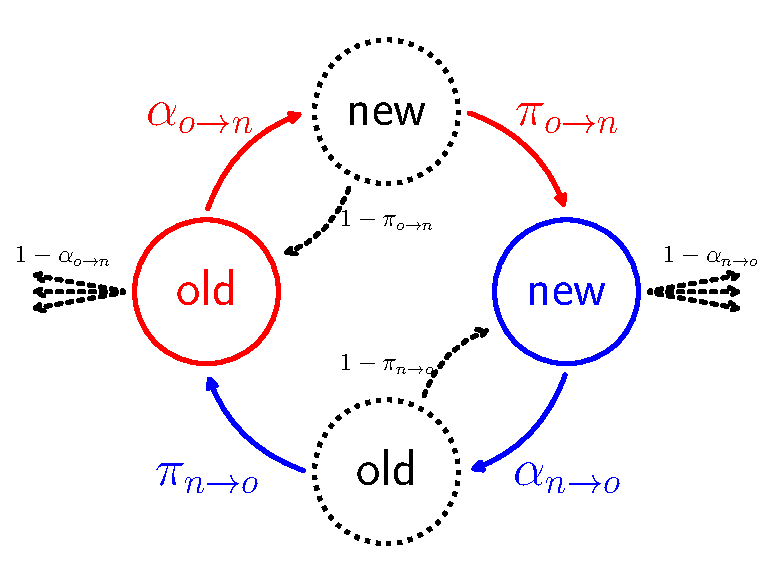
\includegraphics[width=8.5cm]{../figures/detailed_balance.pdf}
\caption{
Probabilities for all possible transitions between two states, old and new, are illustrated.
Proposed configurations and other possible transitions are shown with black dashed circles and arrows, respectively.
Detailed balance is achieved when, for every pair of states, the probability to be in one of the states and then to accept a transition into another state is equal to the probability to be in that other state and then to accept the reverse transition.
}
\label{fig:detailed_balance}
\end{centering}
\end{figure}

In this section, the probability of accepting an attempted MC trial move, or the Metropolis MC trial acceptance probability, denoted by $\chi$, is derived \cite{metropolis_equation_1953, hastings_monte_1970, kofke_monte_1988, allen_computer_1989, frenkel_understanding_2002}.
Ideally, $\chi$ should be close to $1$, so that the trial move in either direction has a high likelihood of being accepted.
The formulation of trial moves is often directed toward this end, while also promoting broader sampling of microstates.

The derivation of $\chi$ in this article requires the condition of detailed balance, shown in Fig.~\ref{fig:detailed_balance}, for a transition from an old microstate, $o$ to a new microstate, $n$,
\begin{equation}
\Pi_o\alpha_{o\rightarrow n}\pi_{o\rightarrow n} = \Pi_n\alpha_{n\rightarrow o}\pi_{n\rightarrow o},
\label{eq:detailed_balance_first}
\end{equation}
where $\Pi_o$ and $\Pi_n$ are the probabilities of being in the old and new microstates, respectively, $\alpha_{o\rightarrow n}$ and $\alpha_{n\rightarrow o}$ are the probabilities of attempting a transition from the old to the new microstate, and vice versa, and $\pi_{o\rightarrow n}$ and $\pi_{n\rightarrow o}$ are the probabilities of accepting those transitions.
Symbols in this article are chosen to follow closely with Ref.~\cite{frenkel_understanding_2002}, but note the different definition of $\pi$.
Detailed balance is a sufficient, but not necessary, condition for ergodic sampling \cite{manousiouthakis_strict_1999}.
For simplicity, we use detailed balance throughout the derivations of this article.
While the microstate probabilities, $\Pi_o$ and $\Pi_n$, are determined solely by the statistical mechanical ensemble, the transition probabilities $\alpha_{o\rightarrow n}$ and $\alpha_{n\rightarrow o}$ depend upon how the MC trial move is implemented.
Thus, Eq.~\ref{eq:detailed_balance_first} provides the route to obtain the trial acceptance probability after the ensemble, trial implementation and acceptance criterion are defined.
Here, \emph{trial implementation} encompasses a great variety of potential moves, such as displacements, volume changes, temperature changes, particle insertions and deletions, alchemical transformations, and more.

In a typical MC simulation, several types of trial moves are employed, with one chosen at random at the beginning of each MC trial.
It is possible that two or more of these trials are capable of producing the same transition between two microstates, albeit in different ways, and with different probabilities.
At first, one might think that the transition probability between two microstates must account for all such ways when determining the acceptance probability $\chi$ to satisfy detailed balance.
Fortunately, this is not the case.
Instead, it is sufficient that each transition method by itself satisfy detailed balance.
It is easy to show that overall detailed balance is satisfied if this ``super-detailed balance" condition is met \cite{frenkel_speed-up_2004}.
In this article, each reversible pair of MC trials is derived as if the pair are the only trials implemented in the simulation.
In special cases, a reversible pair of trials can be obtained by simply repeating the same trial again.
In this special case, the transition probabilities are symmetric.

In general, the Metropolis acceptance criterion is given by,
\begin{equation}
\pi_{o\rightarrow n}=\min(1, \chi),
\end{equation}
where $\chi$ is the Metropolis acceptance probability.
The reverse acceptance probability is $\pi_{n\rightarrow o}=\min(1, 1/\chi)$.
The ratio of $\pi$ is then simplified as,
\begin{equation}
\frac{\pi_{o\rightarrow n}}{\pi_{n\rightarrow o}}=\frac{\min(1, \chi)}{\min(1, 1/\chi)} = \chi,
\label{eq:pi}
\end{equation}
by considering each of the three possibilities, $\chi < 1$, $\chi > 1$ and $\chi=1$, separately.
While the Metropolis acceptance criterion is used throughout this article, other alternatives are possible while maintaining detailed balance.\cite{barker_monte_1965}

Eq.~\ref{eq:detailed_balance_first} may be rearranged to solve for the Metropolis acceptance probability using Eq.~\ref{eq:pi},
\begin{equation}
\chi = \left(\frac{\Pi_n}{\Pi_o}\right)\frac{\alpha_{n\rightarrow o}}{\alpha_{o\rightarrow n}},
\label{eq:detailed_balance}
\end{equation}
where $\chi$ is expressed as the product of two ratios that we refer to throughout this article.

The first ratio in Eq.~\ref{eq:detailed_balance} is the ratio of microstate probabilities, $\Pi_n/\Pi_o$, that may be derived from a given statistical mechanical ensemble, or computed at each step of a converging MC simulation, even if the partition function is not known.
The second ratio may be derived for a given MC trial in a systematic way that is tied very closely to the implementation of the trial.
An important caveat is the ratio $\Pi_n/\Pi_o$ must be expressed in terms of the same set of variables that change during the trial.

%%%%%%%%%%%%%%%%%%%%%%%%%
\section{\label{sec:checklist}Best Practices Checklist for Deriving MC Trial Acceptance}
%%%%%%%%%%%%%%%%%%%%%%%%%

The checklist to obtain MC trial acceptance probabilities in a way that minimizes the possibility of error is provided on the next page.
The acceptance probabilities are derived in a step-by-step manner that is closely related to the simulation algorithms.
By starting from the list of instructions to fully describe a forward and reverse trial, a researcher is able to obtain straightforwardly the required transition probabilities, and identify cases where irreversible changes must be rejected, in a systematic fashion.
We apply this checklist in subsequent sections to derive a variety of unbiased and biased MC trials in various ensembles.
This process of generating the needed acceptance probabilities was inspired by and built upon a set of MC lecture notes \cite{kofke_lecture9_2024} and MC ideal gas simulation tests of various theoretically-based ensemble predictions \cite{hatch_theory_2024}.

\begin{Checklists*}[p!]
\begin{checklist}{Best Practices Checklist for Deriving MC Trial Acceptance}
%\begin{checklist}{\label{sec:checklist}Best Practices Checklist for Deriving MC Trial Acceptance}
\begin{itemize}
\item
  \textbf{Write the MC trial algorithm as an ordered list of all steps required to fully describe both the forward and reverse trials.}

\item
  \textbf{Check detailed balance.}
  \begin{itemize}
    \item Ensure all forward trial steps transition from the old state to a new state.
    \item Consider many different cases, including edge cases such as the largest or smallest values.
    \item Ensure all steps conducted in the reverse trial are capable of returning from the new state to the exact same old state where the forward trial began.
  \end{itemize}

\item
  \textbf{Determine if each step is deterministic, stochastic or needs to be broken into multiple steps.}
  \begin{itemize}
    \item Stochastic steps may choose a particle, position, volume or model parameter.
    \item Stochastic steps make one choice from multiple options.
    \item Stochastic steps often use a random number generator (seeded for reproducibility).
    \item Deterministic steps make no choices.
    \item If more than one choice is made in one step, break that step into multiple steps.
  \end{itemize}

\item
  \textbf{Determine the probability for each step.}
  \begin{itemize}
    \item Determine a probability for choosing a discrete variable (E.g. if the step requires choosing a particle from among $N$ particles, then the probability is $1/N$).
    \item Determine a probability for choosing a continuous variable (E.g., if the step requires choosing a position in a volume $V$, then the probability is $\diff\mathbf{r}/V$).
    \item If the step is deterministic, then the probability is 1.
    \item Determine the forward trial probability, $\alpha_{o \rightarrow n}$, from the old to the new state.
    \item Determine the reverse trial probability, $\alpha_{n \rightarrow o}$, from the new to the old state.
    \item Obtain the total probability of the forward trial as the product of the forward probabilities for each step.
    \item Repeat with the previous step, for the total reverse probability.
  \end{itemize}

\item
  \textbf{Determine the ensemble of the trial.}
  \begin{itemize}
    \item List all possible variables that could change during each step (Note if the particle positions, number of particles, volume or model parameters change).
    \item From the list of all variables that could change, determine the ensemble.
    \item Use $NVT$ ensemble microstate probabilities if only particle positions change.
    \item Use $NPT$ ensemble microstate probabilities if only particle positions and volume change.
    \item Use (semi-)$\mu VT$ ensemble microstate probabilities if the number of particles changes.
    \item Use Gibbs ensemble microstate probabilities if multiple systems are coupled.
    \item Use Expanded ensemble microstate probabilities if temperature or model parameter change (beyond the scope of this article).
  \end{itemize}

\item
  \textbf{Use Eq.~\ref{eq:detailed_balance} to obtain the trial acceptance probability.}
  \begin{itemize}
    \item The ensemble of the trial determines the ratio of microstate probabilities.
    \item The probabilities of each step of the trial implementation determines the ratio of the forward and reverse transition probabilities.
  \end{itemize}

\item
  \textbf{Test the implementation of the trial acceptance probability.}
  \begin{itemize}
    \item Verify that the acceptance probability leads to simulation results that agree with theory and trusted sources.
    \item Start with the simplest possible simulations that are fast, such as ideal gases with tractable theoretical expressions.
  \end{itemize}

\item
  \textbf{Document your derivation or software implementation for later reference.}
  \begin{itemize}
    \item Include documentation and references for future readers (e.g., yourself) to understand the derivation.
  \end{itemize}

\end{itemize}
\end{checklist}
\end{Checklists*}


%%%%%%%%%%%%%%%%%%%%%%%%%
\section{\label{sec:configuration}Description of a configuration with particles, coordinates and periodic boundaries}
%%%%%%%%%%%%%%%%%%%%%%%%%

In this article, a configuration refers to the particles, coordinates and periodic boundaries.
For an $n$-component system, the total number of particles, $N=\sum_{i}^{n} N_i$, where $N_i$ is the number of particles of type $i$.
In bulk systems, there are no interactions of the particles with boundaries.
To avoid spurious effects of walls or a container, and thereby minimizing the size of the simulated system needed to model the bulk, periodic boundary conditions are imposed such that particles interact with their nearest neighboring image \cite{allen_computer_1989}.
To simplify the notation in the following derivations, the periodic boundaries align with the Cartesian axes to form a cuboid of $D$ linear dimensions $L_d$, where the volume, $V$, is given by $V=\prod_d^D L_d$.

The position of each particle is represented by a single vector coordinate $\mathbf{r}$, and all internal and/or orientational coordinates of the particle are represented by a single vector $\boldsymbol{\omega}$.
A particle may be composed of multiple interaction sites that are mutually bound, flexibly or rigidly or both, and the site-site interactions could be orientationally-dependent (e.g., point dipoles).
The orientation of a particle might be given implicitly (not part of $\boldsymbol{\omega}$) via the Cartesian coordinates of its interaction sites.
Alternatively, it may be specified explicitly via an appropriate orientation vector, with the location of the interaction sites (if a multi-site particle) constructed on-the-fly from the position, orientation, and internal coordinates.
In a 3-dimensional space, the orientation coordinate for a cylindrically-symmetric object requires just two independent values, e.g., a unit  vector describing the cylindrical axis direction.
For particles with no such symmetry, three independent values are needed to specify the orientation.
Euler angles are sometimes invoked for this, but they are not particularly useful in the context of molecular simulation.
A better choice is a quaternion, which is a normalized, four-element vector \cite{vesely_angular_1982, karney_quaternions_2007}.

If the particle is not isotropic or rigid, the derivations in this article leave a placeholder variable for the orientation contributions that are not further detailed and are beyond the scope of this article.

%%%%%%%%%%%%%%%%%%%%%%%%%
\section{\label{sec:rhs_nvt}Unbiased canonical ensemble ($NVT$) trials}
%%%%%%%%%%%%%%%%%%%%%%%%%

Canonical-ensemble trials are defined as trials that do not change the total number of particles of each type, $N_i$, the volume, $V$, or the temperature, $T$, and unbiased trials have transition probabilities that do not depend upon the configuration (e.g., not configurational bias).

In order to obtain trial acceptance in the $NVT$ ensemble, first the ratio of microstate probabilities (i.e., the first ratio in Eq.~\ref{eq:detailed_balance}), the probabilities of each microstate must be known proportionally with respect to the variables that change during the trial (e.g., only the coordinates, $\mathbf{r}$).
The probability of a microstate in the $NVT$ ensemble is proportional to \cite{allen_computer_1989, frenkel_understanding_2002}
\begin{equation}
\Pi \diff\mathbf{r}^N\diff\boldsymbol{\omega}^N \propto e^{-\beta U} \diff\mathbf{r}^N\diff\boldsymbol{\omega}^N,
\label{eq:rhs_nvt_pi}
\end{equation}
where $U$ is the total potential energy, $\beta=\frac{1}{k_B T}$, and $k_B$ is the Boltzmann constant.
The integration variables $\diff\mathbf{r}^{N}$ and $\diff\boldsymbol{\omega}^{N}$ are made explicit because these are the variables which change in an $NVT$ trial, and their randomly generated values for perturbations must be chosen uniformly (e.g., for $\diff\mathbf{r}$, choosing uniformly in each dimension, and for $\diff\boldsymbol{\omega}$, choosing uniformly on the surface of a unit sphere).
Because Eq.~\ref{eq:detailed_balance} requires information about only the ratio of microstate probabilities, we do not need to include any coordinate-independent terms that cancel when forming the ratio.
Thus, terms such as the partition function, the thermal de Broglie wavelength and the accounting of indistinguishability do not contribute to the $NVT$ ratio of probabilities.

Given Eq.~\ref{eq:rhs_nvt_pi}, the ratio of $NVT$ microstate probabilities, the first ratio in Eq.~\ref{eq:detailed_balance}, is given by
\begin{equation}
\frac{\Pi_n}{\Pi_o} = e^{-\beta\Delta U},
\label{eq:rhs_nvt}
\end{equation}
where $\Delta U = U_n - U_o$, $U_n$ and $U_o$ are the potential energies of the new and old state, respectively, and $N$, $V$ and $T$ are constant.
This expression is used for any trial that changes only the positions and orientations of the particles.

%%%%%%%%%%%%%%%%%%%%%%%%%
\subsection{\label{sec:lhs_translation}Particle translation trial}
%%%%%%%%%%%%%%%%%%%%%%%%%

An MC translation trial move is defined as follows.
A particle is randomly chosen among all of the mobile, non-fixed particles in the old microstate.
The total number of mobile particles is $N_m=\sum_i^{mobile} N_i$, where $i$ is the particle type.
The randomly chosen particle with position $\mathbf{r}_o$ in the old microstate is then translated by a random amount selected uniformly within $\pm\delta/2$ in each of $D$ dimensions, to a new position labeled $\mathbf{r}_n$, thereby defining the new microstate.

For this trial, the transition probability, $\alpha_{o\rightarrow n}$, may be obtained as the product of the transition probabilities for each step.
Each step that involves the generation of a random number should be considered.
In this translation trial, there are two such steps.
In the first, a particle is chosen randomly among $N_m$ mobile particles.
This means that the probability of choosing that particular particle, $1/N_m$, is the transition probability of the first step.
In the second step, $\mathbf{r}_n$ is chosen uniformly within a region of volume $\delta^D$.
Thus, the transition probability density of choosing $\mathbf{r}_n$ in the second step is $1/\delta^D$, and the transition probability is $\diff\mathbf{r}/\delta^D$.
In a computer experiment, positions may be determined only within machine precision, which is represented here by $\diff\mathbf{r}$.
%In theory, $\diff\mathbf{r}$ is included with the integral of the partition function.
Formally, $\diff\mathbf{r}$ is required to quantify the probability of choosing a position in continuous space.
Thus,
\begin{equation}
\alpha_{o\rightarrow n} = \frac{\diff\mathbf{r}}{N_m \delta^D}.
\label{eq:lhs_disp_forward}
\end{equation}

\begin{figure}
\begin{centering}
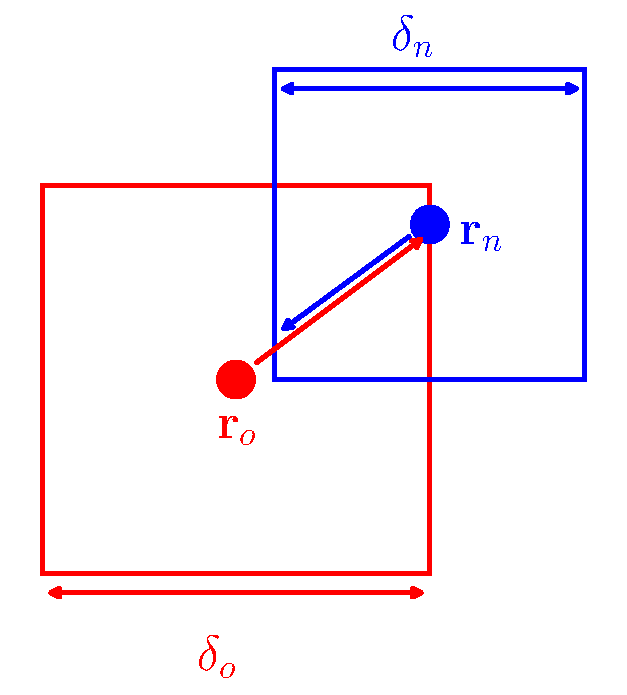
\includegraphics[width=6.5cm]{../figures/lhs_nvt.pdf}
\caption{
Detailed balance is violated if the tunable translation parameter, $\delta$, decreases.
If the particle is translated from the old position, $\mathbf{r}_o$, within $\delta_o$ in each dimension, then the particle may not be able to return to $\mathbf{r}_o$ in the reverse trial if the next translation is within $\delta_n<\delta_o$.
This is why $\delta$ should change only during equilibration and not during production simulations.
}
\label{fig:lhs_nvt}
\end{centering}
\end{figure}

In order to solve for the trial acceptance probability, $\chi$, the reverse trial transition probability from the new microstate to the old microstate, $\alpha_{n\rightarrow o}$, must also be obtained in order to utilize Eq.~\ref{eq:detailed_balance}.
The reverse transition must always be capable of returning to the old microstate; otherwise detailed balance is violated.
For example, detailed balance is violated if $\delta$ is tuned to reach a desired acceptance probability.
When $\delta$ is made smaller after a translation trial, it may be impossible for the next trial to reverse back to the old state, as illustrated in Fig.~\ref{fig:lhs_nvt}.
For this reason, $\delta$ should be changed only during equilibration and not during production simulations.

Throughout this article, we tabulate these forward and reverse transition probabilities, $\pi$, step-by-step with a corresponding table, as shown for a translation trial in Table~\ref{tab:lhs_translation}.
This table should indicate every use of a random number generator in both the forward and reverse transitions.
Again, the overall transition probability for a trial is the product of the probabilities for a given direction.

\begin{table}
\begin{center}
\begin{tabular}{|c|c|c|c|c|}
 \cline{1-2}\cline{4-5}
 \thead{Forward} & \thead{$\alpha_{o\rightarrow n}$} & & \thead{Reverse} & \thead{$\alpha_{n\rightarrow o}$}\\ [0.5ex]
 \cline{1-2}\cline{4-5}
 \makecell{Choose from $N_m$} & \makecell{$1/N_m$} & & \makecell{Choose from $N_m$} & \makecell{$1/N_m$} \\
 \cline{1-2}\cline{4-5}
 \makecell{Choose $\mathbf{r}_n$} & \makecell{$\diff\mathbf{r}/\delta^D$} & & \makecell{Choose $\mathbf{r}_o$} & \makecell{$\diff\mathbf{r}/\delta^D$} \\
 \cline{1-2}\cline{4-5}
\end{tabular}
\caption{Translation transition probabilities.}
\label{tab:lhs_translation}
\end{center}
\end{table}

The reverse transition probability is given by
\begin{equation}
\alpha_{n\rightarrow o} = \frac{\diff\mathbf{r}}{N_m \delta^D}.
\label{eq:lhs_disp_rev}
\end{equation}
Substituting Eqs.~\ref{eq:rhs_nvt}, \ref{eq:lhs_disp_forward} and \ref{eq:lhs_disp_rev} into Eq.~\ref{eq:detailed_balance} yields,
\begin{equation}
\chi = e^{-\beta\Delta U}
\label{eq:lhs_translate}
\end{equation}
for the Metropolis acceptance of translation trials.

\begin{figure}
\lstinputlisting[
language=Python,
label={sim:nvt_harmonic},
caption={MC simulation of a single particle in one dimension attached to a harmonic spring using Python3, where the statistics module is provided in Section~\ref{sec:block_av}. Note that a random number generator seed of "43279857" is provided so that the simulation is reproducible.}
]{../codes/nvt_harmonic.py}
\end{figure}

Code Block~\ref{sim:nvt_harmonic} tests Eq.~\ref{eq:lhs_translate} for a single particle subject to an external harmonic potential centered about the origin in one dimension.
The expected average position is the origin.
Also, according to the equipartition theorem, the expected average energy is $0.5k_BT$.

One major difference between MD and MC is that all particles are moved simultaneously in one MD time step, while typically only a single particle is moved in one MC trial.
If multiple particles were moved in one MC trial, then only one unfavorable overlap from one particle could cause the rejection of an entire trial.
Thus, it is typically more efficient to perturb only one particle at a time.
However, there are special cases where it is still efficient for more than one particle to move in a single trial, as discussed in Section~\ref{sec:lhs_cluster}.

The tunable translation parameter may have an optimal value in a dense fluid.
Larger translations are likely to overlap with another particle, while smaller translations are more correlated with the old microstate, reducing sampling efficiency.
Tunable translation parameters are optimized by changing $\delta$ during an equilibration period to achieve a desired acceptance, often $25$ $\%$ \cite{kolafa_optimization_1987, jacucci_comparing_1984, chapman_metropolis_1985, mountain_quantative_1994, hatch_parallel_2020}.
Although Metropolis \textit{et. al} \cite{metropolis_equation_1953} used 50 \%, it seems that higher efficiencies may be achieved with slightly lower acceptances for particle translation because rejects can be less expensive (e.g., hard overlap detected, updating neighbor lists, etc.) and larger translations can lead to large configuration changes, although too low of acceptance also runs the risk of poor sampling.

An efficient implementation may have a translation parameter, $\delta_i$, specifically tuned for each particle type, $i$.
This could be important to improve sampling in cases where the particle sizes or interactions are different.
In addition, particles are chosen from all mobile particles, $N_m$.
An alternative would be to define separate trials that select among specific particle types.
In that case, if there are more particles of one type than another, the species with fewer numbers could have a relatively larger probability of translation.
The relative efficiency of this alternative approach compared to the one derived here is beyond the scope of this article.
If the minor species is of more interest, the alternative could be more efficient.
On the other hand, inefficiencies could arise if the minor species were caged in solvent that was not as well sampled.
%Although these trials could be assigned different weights to correct this relative probability, such weights would need to be recomputed when the number of particles changes.

The goal of translation trials is to give every particle a chance to move.
In principle, any state may be visited, which is a key element of the ergodic hypothesis.
Although sequential updates have been shown to converge faster than random updates in an Ising model, sequential updates break detailed balance and follow a weaker balance condition \cite{ren_acceleration_2006}.
Trials that do not obey detailed balance are outside the scope of this article.

This translation algorithm could also be carefully modified to select particles only in a specific region of space.
But detailed balance violations could occur if the set of available particles changes.
For example, it is possible for the translation to take a particle out of this region.
If so, the trial must be immediately rejected, because the particle that was taken out of the region cannot be chosen for the reverse transition and therefore detailed balance is violated.

%%%%%%%%%%%%%%%%%%%%%%%%%
\subsection{\label{sec:lhs_rotation}Particle orientation-change trial}
%%%%%%%%%%%%%%%%%%%%%%%%%

Orientations are typically fixed during particle translation trials so as not to introduce a second tunable parameter for orientation moves that cannot be decoupled from the translation parameter during optimization.
Instead, the orientation of a single particle may be perturbed in a separate trial move.
A robust and intuitive way to accomplish this is via the axis-angle method: (1) a particle is randomly chosen among $N_m$ mobile particles; (2) a rotation axis $\hat {\bf u}$ is generated by sampling uniformly on the surface of a sphere (Sec.~\ref{sec:unit_sphere}); (3) a rotation angle $\theta$ is generated uniformly on $\pm\delta\theta_{max}/2$ (with $\delta\theta_{max}$ a tunable parameter).
With the rotation so defined, a rotation matrix can be computed
\begin{equation}
\mathbf{R} =
\begin{bmatrix}
C + (1 - C) u_x^2 & (1 - C) u_x u_y - S u_z & (1 - C) u_x u_z + S u_y \\
(1 - C) u_y u_x + S u_z & C + (1 - C) u_y^2 & (1 - C) u_y u_z - S u_x \\
(1 - C) u_z u_x - S u_y & (1 - C) u_z u_y + S u_x & C + (1 - C) u_z^2
\end{bmatrix}
\label{eq:rotation_matrix}
\end{equation}
where $C =\cos\theta$ and $S = \sin\theta$.
The new coordinate of interaction site $j$ on particle $i$ at ${\bf r}_i$ is given by ${{\bf r}_{ij,{\rm n}}={\bf r}_{i}}+{\mathbf R}({\bf r}_{ij,{\rm o}}-{\bf r}_i)$.
If the particle's centroid is chosen for ${\bf r}_i$, then the centroid will be unchanged by the rotation (complementing the translation move, which leaves the orientation unchanged).
However, using the centroid for ${\bf r}_i$ is not a requirement; any well-defined center for the rotation may be employed (e.g., the position of a specific interaction site).

Alternatively, if the orientation coordinate is held explicitly (e.g., as a quaternion), then it can be updated from $\hat{\bf u}$ and $\theta$ using an appropriate formula.

%Axis-angle is suitable for orientation displacement of particles of any symmetry. However, it is not suitable for generating a random orientation from scratch, i.e. by selecting $\delta = 2\pi$. Generating a random quaternion is best for this.
Regardless of the selected center for the rotation, the transition probabilities are given in terms of the axis-angle selection process outlined above.
The elements of the transition probabilities for the particle orientation trial are summarized in Table~\ref{tab:lhs_rotation}.
Together they yield the forward and reverse probabilities, which in this case are again equal
\begin{equation}
  \alpha_{o\rightarrow n}=\alpha_{n\rightarrow o} = \frac{\diff\mathbf{\omega}\diff\theta}{N_m 4\pi\delta\theta_{max}}.
\label{eq:lhs_rhs_rot_fwdrev}
\end{equation}

\begin{table}
\begin{center}
\begin{tabular}{|c|c|}
 \hline
 \thead{Forward} & \thead{$\alpha_{o\rightarrow n}$} \\ [0.5ex]
 \hline
 \makecell{Choose from $N_m$} & \makecell{$1/N_m$} \\
 \hline
 \makecell{Choose rotation axis} & \makecell{$\diff\boldsymbol{\omega}/4\pi$} \\
 \hline
  \makecell{Choose rotation angle} & \makecell{$\diff\theta/\delta\theta_{max}$} \\
 \hline\hline
 \thead{Reverse} & \thead{$\alpha_{n\rightarrow o}$}\\ [0.5ex]
 \hline
 \makecell{Choose from $N_m$} & \makecell{$1/N_m$} \\
 \hline
 \makecell{Choose rotation axis} & \makecell{$\diff\boldsymbol{\omega}/4\pi$} \\
 \hline
  \makecell{Choose rotation angle} & \makecell{$\diff\theta/\delta\theta_{max}$} \\
 \hline
\end{tabular}
\caption{Orientation-change transition probabilities.}
\label{tab:lhs_rotation}
\end{center}
\end{table}

Substituting Eq.~\ref{eq:rhs_nvt} into Eq.~\ref{eq:detailed_balance} and using the transition probabilities in Table~\ref{tab:lhs_rotation} yields,
\begin{equation}
\chi = e^{-\beta\Delta U}
\label{eq:lhs_rotate}
\end{equation}
for the Metropolis acceptance of particle orientation changes.
To simplify notation, all remaining trial moves which include changes in orientation will simply refer to these transition probabilities as $P_{\omega n}$ and $P_{\omega o}$ for the new and old states, respectively.

A larger tunable parameter, $\delta\theta_{max}$, leads to a larger rotation, and thus $\delta\theta_{max}$ may be tuned in the same manner as the translation tunable parameter to reach a target acceptance for each species.
To avoid violating detailed balance, this tunable parameter should remain constant during the production simulations for the same reason as shown in Fig.~\ref{fig:lhs_nvt}.

If desired, generation of orientations from scratch, without perturbing on an existing orientation, is best accomplished by random generation of a quaternion.
An example of randomly picking quaternions, and thus orientations, is shown in Section~\ref{sec:unit_sphere}.

Code Block~\ref{sim:orientation_trials} tests Eqs.~\ref{eq:rotation_matrix} and \ref{eq:lhs_rotate} with the simulation of the orientation of a single rigid body given by two orthogonal unit vectors in $3$ dimensions.
Because there is no energy of interaction, the unit vectors are expected to be uniformly distributed on the surface of a sphere.
In spherical coordinates, this manifests as a uniform distribution of the azimuthal angle $\in [-\pi,\pi]$, which is defined as the angle between the x-axis and the projection of the vector on the x-y plane, and a sine distribution for the polar angle $\in [0,\pi]$, which is the angle between the z-axis and the vector.
While this azimuthal and polar angle of the first vector fully specifies the orientations of rigid bodies with an axis of symmetry, generic rigid bodies also require analysis of a third angle.
That third angle was chosen to be the azimuthal angle of the second vector in the reference frame of the first vector.
The reference frame was defined by the minimal rotation of the coordinate axes such that the z-axis aligns with the first vector.
These analytical expectations are compared against the MC simulation in Fig.~\ref{fig:orientation_trials}.

\begin{figure}
\lstinputlisting[
language=Python,
label={sim:orientation_trials},
caption={MC simulation of a single rigid body represented by two orthogonal unit vectors in three dimensions implemented in Python 3 using $5\times 10^5$ random angular displacements with $\delta\theta_{max}=\pi/10$. Angle distributions were computed over $300$ equally-spaced bins with $20$ independent simulations (totaling $10^7$ MC trials) to compare against theoretical expectations with approximately 68 \% of the distribution within one standard deviation.}
]{../codes/orientation_trials.py}
\end{figure}

\begin{figure}
\begin{centering}
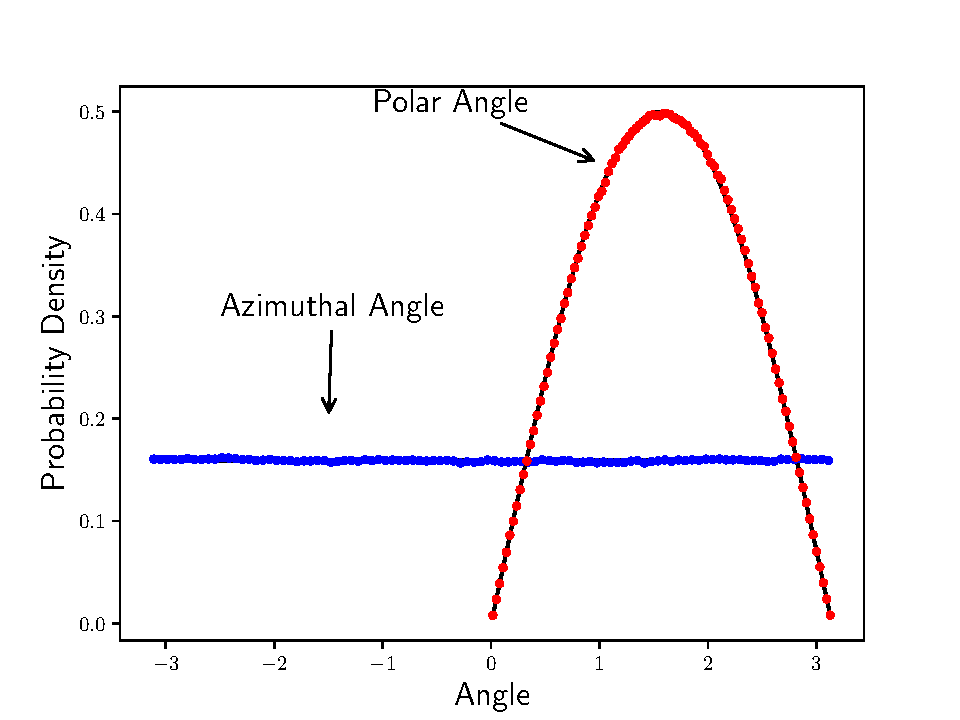
\includegraphics[width=8.5cm]{../figures/orientation_trials.pdf}
\caption{
  The (blue) azimuthal and (red) polar probability distributions of the first vector and (orange) azimuthal angle of the second vector in the reference frame of the first vector from MC simulations described in Code Block~\ref{sim:orientation_trials} with error bars from the standard deviation of the mean of $20$ independent simulations, and analytical expectations shown by the black lines.
\label{fig:orientation_trials}
}
\end{centering}
\end{figure}
%If desired, generation of orientations from scratch, without perturbing on an existing orientation, is accomplished by random generation of a quaternion \cite{vesely_angular_1982}.
%An example of randomly picking quaternions, and thus orientations, is shown in Section~\ref{sec:unit_sphere}.

%As a simple example, consider choosing a second site of a dimer that is bonded to the first with $k$ randomly generated positions according to the Boltzmann weighted potential, $U_{bond}$.
%In this case,
%\begin{equation}
%P_{\omega n}=\frac{e^{-\beta U_{bond}}}{W_n}
%\label{eq:pomegan}
%\end{equation}
%\begin{equation}
%W_n = \sum_k e^{-\beta U_{bond,k}}.
%\end{equation}
%Substituting Eq.~\ref{eq:pomegan} into \ref{eq:lhs_rotate}
%where the numerator removes the bonded energy from the total energy in Eq.~\ref{eq:lhs_rotate} so that only intermolecular energies are considered in the final acceptance, and the denominator is the usual Rosenbluth factor.

%%%%%%%%%%%%%%%%%%%%%%%%%
\section{\label{sec:rhs_npt}Unbiased isothermal-isobaric ensemble trials}
%%%%%%%%%%%%%%%%%%%%%%%%%

Isothermal-isobaric ensemble trials change the volume, $V$, with constant number of particles, $N$, pressure, $P$ and temperature, $T$.
Volume-change trials are conducted while simultaneously scaling the coordinates of the particles uniformly.
This is done for a variety of reasons that are discussed in Section~\ref{sec:lhs_dv}.
In order to derive the appropriate MC acceptance criteria for this trial, the microstate probability must be expressed in scaled coordinates given by $s_d = r_d/L_d$, where $d$ is the dimensionality of the system.
In the following two sections, we consider the $NPT$ ensemble both without and with a ``shell" particle~\cite{koper_length_1996, corti_deriving_1998, hatch_theory_2024}, where a shell particle is used to remove redundant microstates from the isothermal-isobaric ensemble partition function.

%%%%%%%%%%%%%%%%%%%%%%%%%
\subsection{\label{sec:rhs_npt_shell}Isothermal-isobaric ($NPT$) ensemble without a shell particle}
%%%%%%%%%%%%%%%%%%%%%%%%%

The microstate probability in the $NPT$ ensemble without a shell particle is proportional to \cite{wood_monte_1968, allen_computer_1989, frenkel_understanding_2002}
\begin{equation}
\Pi \diff\mathbf{s}^{N}\diff\boldsymbol{\omega}^{N}\diff V \propto V^{N} e^{-\beta(U+P V)} \diff\mathbf{s}^{N} \diff\boldsymbol{\omega}^{N}\diff V.
\label{eq:rhs_npt_pi}
\end{equation}
The ratio of microstate probabilities, the first ratio in Eq.~\ref{eq:detailed_balance}, is given by
\begin{equation}
\frac{\Pi_n}{\Pi_o} = \left(\frac{V_n}{V_o}\right)^{N}e^{-\beta(\Delta U + P\Delta V)},
\label{eq:rhs_npt_delta_v}
\end{equation}
for trials that select random changes uniformly in $V$, because $V$ is the explicit variable in Eq.~\ref{eq:rhs_npt_pi}.
If an $NVT$ trial is attempted in the $NPT$ ensemble, $\Delta V=0$, and Eq.~\ref{eq:rhs_npt_pi} reduces to Eq.~\ref{eq:rhs_nvt}.

Eq.~\ref{eq:rhs_npt_pi} and \ref{eq:rhs_npt_delta_v} no longer apply if changes are uniform in $\ln V$ instead of $V$.
In this case, substituting $\diff V=V\diff\ln V$ into Eq.~\ref{eq:rhs_npt_pi}, the first ratio in Eq.~\ref{eq:detailed_balance} is
\begin{equation}
\frac{\Pi_n}{\Pi_o} = \left(\frac{V_n}{V_o}\right)^{N+1}e^{-\beta(\Delta U + P\Delta V)}.
\label{eq:rhs_npt_delta_lnv}
\end{equation}
See Code Block~\ref{sim:ideal_gas_npt} for a test of Eqs.~\ref{eq:rhs_npt_delta_v} and \ref{eq:rhs_npt_delta_lnv}.

%%%%%%%%%%%%%%%%%%%%%%%%%
\subsection{\label{sec:lhs_dv}Isotropic volume change trial}
%%%%%%%%%%%%%%%%%%%%%%%%%

Trial moves that attempt isotropic volume changes proceed as follows.
The positions of the particles and periodic boundary lengths are scaled by a factor of $(1+\Delta V/V_o)^{1/D}$ in each of $D$ dimensions, where $\Delta V$ is chosen as a random amount selected uniformly within $\pm\Delta V_{\mathrm{max}}$.
The particle positions are typically scaled with the volume in off lattice simulations.
Careful consideration of exactly how volume is changed is required.
For example, as shown in Fig.~\ref{fig:npt}, if particle positions are wrapped during volume changes that do not scale the positions, then detailed balance may be violated.
This trial is summarized in Table~\ref{tab:lhs_dv}.

\begin{figure}
\begin{centering}
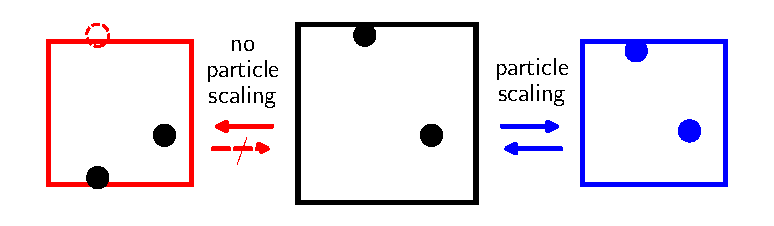
\includegraphics[width=8.5cm]{../figures/npt.pdf}
\caption{
Detailed balance is violated if the particle positions are not scaled with the volume and one of the particles is wrapped across periodic boundaries.
On the left, the top-most particle is wrapped to the bottom due to the decrease in volume when particle positions are not scaled.
The reverse move, a subsequent increase in volume without scaling, will not return the system to its original microstate, shown in the center.
On the right, detailed balance is obeyed when the particle positions are scaled with the volume.
}
\label{fig:npt}
\end{centering}
\end{figure}

\begin{table}
\begin{center}
\begin{tabular}{|c|c|}
 \hline
 \thead{Forward} & \thead{$\alpha_{o\rightarrow n}$} \\ [0.5ex]
 \hline
 \makecell{Choose $\Delta V$} & \makecell{$\diff\mathbf{r}/(2\Delta V_{\mathrm{max}})$} \\
 \hline\hline
 \thead{Reverse} & \thead{$\alpha_{n\rightarrow o}$}\\ [0.5ex]
 \hline
 \makecell{Choose $-\Delta V$} & \makecell{$\diff\mathbf{r}/(2\Delta V_{\mathrm{max}})$} \\
 \hline
\end{tabular}
\caption{Volume change transition probabilities.}
\label{tab:lhs_dv}
\end{center}
\end{table}

Substituting Eq.~\ref{eq:rhs_npt_delta_v} (without a shell particle) into Eq.~\ref{eq:detailed_balance}, and using Table~\ref{tab:lhs_dv} for the second ratio in Eq.~\ref{eq:detailed_balance} results in
\begin{equation}
\chi=\left(\frac{V_n}{V_o}\right)^{N}e^{-\beta(\Delta U + P\Delta V)}.
\label{eq:lhs_dv}
\end{equation}
This equation is also valid for uniform changes in one of the side lengths, $L_d$, with scaled particle positions because $dV \propto \diff L_d$ in Eq.~\ref{eq:rhs_npt_pi} results in the same Eq.~\ref{eq:rhs_npt_delta_v} for the first ratio in Eq.~\ref{eq:detailed_balance}.

Eq.~\ref{eq:lhs_dv} is not valid for uniformly random changes in $\ln V$.
Specifically, uniform changes in $\ln V$ occur when the particle coordinates and periodic boundary lengths are scaled by a factor of $e^{(\delta\ln V)/D}$, where $\delta\ln V$ is chosen as a random amount selected uniformly within $\pm\delta\ln V_{\mathrm{max}}$, and $\Delta V = V_o(e^{\delta\ln V}-1)$.
As discussed in Ref.~\cite{frenkel_understanding_2002} (without a shell particle) and Ref.~\cite{corti_monte_2002} and Section~\ref{sec:rhs_npt} (with a shell particle), uniform changes in $\ln V$ use Eq.~\ref{eq:rhs_npt_delta_lnv} instead of Eq.~\ref{eq:rhs_npt_delta_v}, resulting in the following acceptance probability
\begin{equation}
\chi=\left(\frac{V_n}{V_o}\right)^{N+1}e^{-\beta(\Delta U + P\Delta V)}.
\label{eq:lhs_dlnv}
\end{equation}
Code Block~\ref{sim:ideal_gas_npt} uses Eq.~\ref{eq:lhs_dv} or Eq.~\ref{eq:lhs_dlnv} for an ideal gas to compare against theory for uniform changes in $V$ or $\ln V$, respectively.

\begin{figure}
\lstinputlisting[
language=Python,
label={sim:ideal_gas_npt},
caption={MC simulation of an ideal gas in the $NPT$ ensemble using Python3 with a shell particle and uniform changes in $V$ or $\ln V$, and the statistics module is provided in Section~\ref{sec:block_av}.}
]{../codes/ideal_gas_npt.py}
\end{figure}

%%%%%%%%%%%%%%%%%%%%%%%%%
\subsection{\label{sec:rhs_npt_no_shell}Isothermal-isobaric ensemble with a shell particle}
%%%%%%%%%%%%%%%%%%%%%%%%%

If a shell particle is introduced to remove redundant microstates in the partition function~\cite{attard_density_1995, koper_length_1996, corti_deriving_1998, han_isothermal-isobaric_2001, corti_isothermal-isobaric_2001, corti_monte_2002, stroker_systematic_2021, hatch_theory_2024}, then there is one less particle that is scaled by the volume and Eqs.~\ref{eq:rhs_npt_pi}, \ref{eq:rhs_npt_delta_v} and \ref{eq:rhs_npt_delta_lnv} become 
\begin{equation}
\Pi \diff\mathbf{s}^{N-1}\diff\boldsymbol{\omega}^{N}\diff V \propto V^{N-1} e^{-\beta(U+P V)} \diff\mathbf{s}^{N-1} \diff\boldsymbol{\omega}^{N}\diff V,
\end{equation}
\begin{equation}
\frac{\Pi_n}{\Pi_o} = \left(\frac{V_n}{V_o}\right)^{N-1}e^{-\beta(\Delta U + P\Delta V)},
\end{equation}
and
\begin{equation}
\frac{\Pi_n}{\Pi_o} = \left(\frac{V_n}{V_o}\right)^{N}e^{-\beta(\Delta U + P\Delta V)},
\end{equation}
respectively.
The acceptance probabilities shown in Section \ref{sec:lhs_dv} without a shell particle would change according to these new microstate probabilities when a shell particle is included.
Specifically, Eqs.~\ref{eq:lhs_dv} and \ref{eq:lhs_dlnv} become
\begin{equation}
\chi=\left(\frac{V_n}{V_o}\right)^{N-1}e^{-\beta(\Delta U + P\Delta V)}.
\end{equation}
and
\begin{equation}
\chi=\left(\frac{V_n}{V_o}\right)^{N}e^{-\beta(\Delta U + P\Delta V)},
\end{equation}
for uniform changes in $V$ and $\ln V$, respectively.

%%%%%%%%%%%%%%%%%%%%%%%%%
\section{\label{sec:rhs_muvt}Unbiased grand canonical ensemble ($\mu VT$) trials}
%%%%%%%%%%%%%%%%%%%%%%%%%

In this section, we will derive insertion and deletion trials in two cases.
In the first case, distinguishable particles in unscaled coordinates are considered.
In the second case, indistinguishable particles in scaled coordinates are considered.
Both cases will be shown to have identical acceptance probabilities.

%%%%%%%%%%%%%%%%%%%%%%%%%
\subsection{\label{sec:rhs_muvt_distinguishable}Grand canonical ensemble with distinguishable particles in unscaled coordinates}
%%%%%%%%%%%%%%%%%%%%%%%%%

A $\mu VT$ trial changes the number of particles of type $i$, given by $N_i$ with constant chemical potential, $\mu_i$, constant number of other particles, $N-N_i$, volume, $V$ and temperature, $T$.
The $\mu VT$ probability of a microstate is given by \cite{norman_investigation_1969, adams_grand_1975, allen_computer_1989, frenkel_understanding_2002}
\begin{equation}
\Pi(N_i) \diff\mathbf{r}^N \diff\boldsymbol{\omega}^N\propto \frac{e^{\beta\mu_i N_i - \beta U}}{\Lambda_i^{DN_i}} \diff\mathbf{r}^N\diff\boldsymbol{\omega}^N,
\label{eq:rhs_muvt_pi}
\end{equation}
where $\Lambda_i$ is the de Broglie wavelength of species $i$.
In classical computer experiments, the particles are treated as distinguishable (e.g., each particle is distinguished by an index in an ordered array).
In this case, the indistinguishable particle correction of $1/N!$ does not appear.
We will show that identical acceptance probabilities are obtained whether we treat the particles as distinguishable or indistinguishable by including the $N!$ term in an alternative derivation in the following Section~\ref{sec:rhs_muvt_alt}.

It is convenient to make Eq.~\ref{eq:rhs_muvt_pi} more compact by introducing the activity, $z_i$, of a particle of type $i$,
\begin{equation}
z_i = \frac{e^{\beta \mu_i}}{\Lambda_i^D}.
\label{eq:activity}
\end{equation}
which has the units of inverse volume and is equivalent to the ideal gas number density.
The number of particles of type $i$ in an ideal gas, $N_{i}^{\mathrm{id}}$, may be derived as the partial derivative of the grand potential with respect to the chemical potential of $i$ at constant $V$ and $T$, resulting in
\begin{equation}
N_{i}^{\mathrm{id}} = V\frac{e^{\beta \mu_i}}{\Lambda_i^D} = Vz_i.
\label{eq:gce_ideal_gas_density}
\end{equation}
Substituting Eq.~\ref{eq:activity} into Eq.~\ref{eq:rhs_muvt_pi} results in
\begin{equation}
\Pi(N_i) \diff\mathbf{r}^N \diff\boldsymbol{\omega}^N\propto z_i^{N_i} e^{-\beta U} \diff\mathbf{r}^N\diff\boldsymbol{\omega}^N.
\label{eq:rhs_muvt_pi_z}
\end{equation}
Using Eq.~\ref{eq:rhs_muvt_pi_z}, the ratio of $\mu VT$ microstate probabilities in Eq.~\ref{eq:detailed_balance} is given by
\begin{equation}
\frac{\Pi_n}{\Pi_o} = (z_i\diff\mathbf{r}\diff\boldsymbol{\omega})^{\Delta N_i} e^{-\beta\Delta U}.
\label{eq:rhs_muvt}
\end{equation}
where $\Delta N_i = N_{in} - N_{io}$, and $N_{in}$ and $N_{io}$ are the number of particles of type $i$ in the new and old microstate, respectively.
If an $NVT$ trial is attempted in the $\mu VT$ ensemble, $\Delta N_i=0$, and Eq.~\ref{eq:rhs_muvt} is reduced to Eq.~\ref{eq:rhs_nvt}.

%%%%%%%%%%%%%%%%%%%%%%%%%
\subsection{\label{sec:lhs_insdel}Insertion and deletion trials with distinguishable particles in unscaled coordinates}
%%%%%%%%%%%%%%%%%%%%%%%%%

\begin{figure}
\begin{centering}
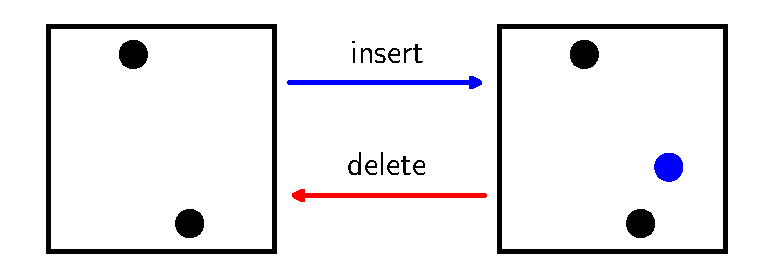
\includegraphics[width=8.5cm]{../figures/muvt.pdf}
\caption{
Insertion trials randomly add a particle, here shown in blue, uniformly within the simulation volume.
Deletion trials remove a random particle, and are the reverse of insertions.
}
\label{fig:muvt}
\end{centering}
\end{figure}

Because particle insertion and deletion trials \cite{norman_investigation_1969, adams_grand_1975} are the reverse of each other, as shown in Fig.~\ref{fig:muvt}, they must be considered together to derive the acceptance probability.
These two trials are collectively referred to as particle transfers (from an ideal gas state).
Insertion and deletion trials for particles of type $i$ proceed as follows.
First, a particle insertion or deletion trial is chosen with equal probability.\footnote{More generally, insertions may be selected with a probability of $P_{bias}$ that is not necessarily $1/2$, and deletions with a probability of $1-P_{bias}$.
In multiple places in this article, we use a $1/2$ probability for choosing between two different trials to simplify the equations.}
If a particle insertion trial is chosen, then a particle type $i$ is placed at a random position selected uniformly in the simulation volume, $V$.
If a particle deletion trial is chosen, then a particle of type $i$ is randomly chosen from among the $N_i$ particles for removal.
If multiple particle types are to be inserted and deleted, then the MC simulation could have a trial for each particle type.

In order to apply Eq.~\ref{eq:detailed_balance}, reverse trials must be considered as having occurred immediately after the forward trial.
This is important to note when deriving the probability of the reverse move, and to clarify that $N_i$ is defined at the beginning of the insertion trial.
The reverse trial deletion then has $N_i+1$ particles of type $i$, including the particle that was added during the forward transition.
Transition probabilities for insertion and deletion are not symmetric \cite{norman_investigation_1969, hastings_monte_1970}.
The transition probability of an insertion trial as the forward transition is then summarized in Table~\ref{tab:lhs_ins}.

\begin{table}
\begin{center}
\begin{tabular}{|c|c|}
 \hline
 \thead{Forward} & \thead{$\alpha_{o\rightarrow n}$} \\ [0.5ex]
 \hline
 Choose insert & $1/2$ \\
 \hline
 Choose position in $V$ & $\diff\mathbf{r}/V$ \\
 \hline
 Choose orientation & $P_{\omega n}\diff\boldsymbol{\omega}$ \\
 \hline\hline
 \thead{Reverse} & \thead{$\alpha_{n\rightarrow o}$} \\ [0.5ex]
 \hline
 Choose delete & $1/2$ \\
 \hline
 Choose particle of type $i$ & $1/(N_i+1)$ \\
 \hline
\end{tabular}
\caption{Particle insertion transition probabilities.}
\label{tab:lhs_ins}
\end{center}
\end{table}

Substituting Eq.~\ref{eq:rhs_muvt} into the first ratio in Eq.~\ref{eq:detailed_balance}, and using Table~\ref{tab:lhs_ins} for the second ratio in Eq.~\ref{eq:detailed_balance} results in
\begin{equation}
\chi = \frac{V z_i}{P_{\omega n}(N_i+1)}e^{-\beta\Delta U},
\label{eq:lhs_ins}
\end{equation}
where $P_{\omega n}=1$ (or incorporated into the definition of $z_i$) if a completely random orientation of a rigid body is chosen (see Section~\ref{sec:lhs_rotation}), or is otherwise related to the Rosenbluth factor in CB partial regrowth of the particle (as discussed in Section~\ref{sec:lhs_rotation}).

Now consider the deletion as the forward transition.
Deletion acceptance is nearly identical to what arises for the reverse of insertions, with one caveat.
With insertion as the forward transition, $N_i$ was defined at the beginning of the insertion trial (e.g., the old microstate, or before the particle was inserted).
For deletion as the forward transition, the old microstate has $N_i$ particles to choose among.
To summarize, the transition probabilities with deletion as the forward transition and insertion as the reverse is given in Table~\ref{tab:lhs_del}.

\begin{table}
\begin{center}
\begin{tabular}{|c|c|}
 \hline
 \thead{Forward} & \thead{$\alpha_{o\rightarrow n}$} \\ [0.5ex]
 \hline
 Choose delete & $1/2$ \\
 \hline
 Choose particle of type $i$ & $1/N_i$ \\
 \hline\hline
 \thead{Reverse} & \thead{$\alpha_{n\rightarrow o}$} \\ [0.5ex]
 \hline
 Choose insert & $1/2$ \\
 \hline
 Choose position in $V$ & $\diff\mathbf{r}/V$ \\
 \hline
 Choose orientation & $P_{\omega o}\diff\boldsymbol{\omega}$ \\
 \hline
\end{tabular}
\caption{Particle deletion transition probabilities.}
\label{tab:lhs_del}
\end{center}
\end{table}

Thus, the acceptance probability for deletions is given by
\begin{equation}
\chi = \frac{P_{\omega o} N_i}{Vz_i}e^{-\beta\Delta U},
\label{eq:lhs_del}
\end{equation}
where $P_{\omega o}=1$ (or incorporated into the definition of $z_i$) if rigid bodies are inserted with random orientations, or otherwise related to the Rosenbluth factor in CB \cite{frenkel_understanding_2002}.
Code Block~\ref{sim:ideal_gas_muvt} uses Eqs.~\ref{eq:lhs_ins} and \ref{eq:lhs_del} for an ideal gas to compare against theory, Eq.~\ref{eq:gce_ideal_gas_density}.

\begin{figure}
\lstinputlisting[
language=Python,
label={sim:ideal_gas_muvt},
caption={MC $\mu VT$ simulation of an ideal gas using Python3, and the statistics module is provided in Section~\ref{sec:block_av}.}
]{../codes/ideal_gas_muvt.py}
\end{figure}

%%%%%%%%%%%%%%%%%%%%%%%%%
\subsection{\label{sec:rhs_muvt_alt}Grand canonical ensemble with indistinguishable particles in scaled coordinates}
%%%%%%%%%%%%%%%%%%%%%%%%%

Consider an alternative approach that includes the indistinguishable particle $N!$ correction, and uses scaled coordinates, as described in Ref.~\cite{frenkel_understanding_2002}.
In this case, the $\mu VT$ microstate probability is
\begin{equation}
\Pi(N_i)\diff\mathbf{s}^{N}\diff\boldsymbol{\omega}^{N} \propto \frac{V^{N}z_i^{N_i}}{N!} e^{-\beta U} \diff\mathbf{s}^{N}\diff\boldsymbol{\omega}^{N}.
\end{equation}
The ratio of $\mu VT$ microstate probabilities for the special case of indistinguishable particles and scaled coordinates is then
\begin{equation}
\frac{\Pi_n}{\Pi_o} = \frac{N_{io}!}{N_{in}!}\left(V z_i\diff\mathbf{s}\diff\boldsymbol{\omega}\right)^{\Delta N_i}e^{-\beta\Delta U},
\label{eq:rhs_muvt_alt}
\end{equation}
and is valid for changing the number of indistinguishable particles and choosing a newly inserted particle position in scaled coordinates, $\mathbf{s}$, not $\mathbf{r}$.


%%%%%%%%%%%%%%%%%%%%%%%%%
\subsection{\label{sec:lhs_insdel_alt}Insertion and deletion trials with indistinguishable particles in scaled coordinates}
%%%%%%%%%%%%%%%%%%%%%%%%%

As opposed to deriving insertion and deletion acceptances with distinguishable particles in non-scaled coordinates, as in Sections~\ref{sec:rhs_muvt_distinguishable} and \ref{sec:lhs_insdel}, consider a similar trial conducted with indistinguishable particles in scaled coordinates, as in Ref.~\cite{frenkel_understanding_2002}.
In this case, the first ratio in Eq.~\ref{eq:detailed_balance} is given by Eq.~\ref{eq:rhs_muvt_alt}.
But since the transition probabilities also change, the same acceptances are nonetheless obtained.

The insertion and deletion trial proceeds as follows.
First, a particle insertion or deletion trial is randomly chosen with equal probability.
If a particle insertion is chosen, then a particle of a given type $i$ is placed at a random position selected uniformly in the scaled coordinates with a probability of $\diff\mathbf{s}$.
If a particle deletion is chosen, then a random particle of a given type is chosen for removal.
Because the particles are indistinguishable, the probability associated with the selection of a particle is $1$.
The forward and reverse transitions are summarized in Table~\ref{tab:lhs_insdel_alt}.

\begin{table}
\begin{center}
\begin{tabular}{|c|c|}
 \hline
 \thead{Forward} & \thead{$\alpha_{o\rightarrow n}$} \\ [0.5ex]
 \hline
 Choose insert & $1/2$ \\
 \hline
 Choose position in scaled coordinates & $\diff\mathbf{s}$ \\
 \hline
 Choose orientation & $P_{\omega n}\diff\boldsymbol{\omega}$ \\
 \hline\hline
 \thead{Reverse} & \thead{$\alpha_{n\rightarrow o}$} \\ [0.5ex]
 \hline
 Choose delete & $1/2$ \\
 \hline
 Choose from indistinguishable particles & $1$ \\
 \hline
\end{tabular}
\caption{Alternative particle insertion transition probabilities.}
\label{tab:lhs_insdel_alt}
\end{center}
\end{table}

The product of the first and second ratios in Eq.~\ref{eq:detailed_balance} is then identical to Eq.~\ref{eq:lhs_ins} because the first ratio from Eq.~\ref{eq:rhs_muvt_alt} now supplies the terms missing from the second ratio.
Thus, the use of indistinguishable particles and scaled coordinates shifts the terms from the transition probabilities to the microstate probabilities.
Although either approach is equally valid, the remainder of this article uses distinguishable particles, as implemented in computer simulations, and $\mu VT$ derivations will use unscaled coordinates as described in Section~\ref{sec:rhs_muvt_distinguishable}, and not Section~\ref{sec:rhs_muvt_alt}.


%%%%%%%%%%%%%%%%%%%%%%%%%
\section{\label{sec:rhs_smuvt}Unbiased semi-grand canonical (semi-$\mu VT$) ensemble trials}
%%%%%%%%%%%%%%%%%%%%%%%%%

Semi-$\mu VT$ trials have fixed total numbers of particles, but the composition may change \cite{kofke_monte_1988}.
For a trial in which particles of type $i$ may be replaced with particles of type $j$, and vice versa, the probability of a microstate in the semi-$\mu VT$ ensemble is proportional to \cite{kofke_monte_1988}
\begin{equation}
\Pi(N_i,N_j) \diff\mathbf{r}^N \diff\boldsymbol{\omega}^N\propto z_i^{N_i} z_j^{N_j} e^{-\beta U} \diff\mathbf{r}^N\diff\boldsymbol{\omega}^N.
\label{eq:rhs_smuvt_pi}
\end{equation}
Using Eq.~\ref{eq:rhs_smuvt_pi}, the ratio of microstate probabilities of the semi-$\mu VT$ ensemble in Eq.~\ref{eq:detailed_balance} is given by
\begin{equation}
\frac{\Pi_n}{\Pi_o} = z_i^{\Delta N_i}z_j^{\Delta N_j} e^{-\beta\Delta U}.
\label{eq:rhs_sgcmc}
\end{equation}
with the constraint that $\Delta N_i + \Delta N_j = 0$.

%%%%%%%%%%%%%%%%%%%%%%%%%
\subsection{\label{sec:lhs_sgcmc}Changing particle type}
%%%%%%%%%%%%%%%%%%%%%%%%%

The semi-$\mu VT$ ensemble described in Section~\ref{sec:rhs_smuvt} allows particles of one type to change into another, as shown in Fig.~\ref{fig:sgcmc}.
A particle type change trial proceeds as follows.
First, the trial is defined with a number of particle types, $n$ that many change into each other.
Thus, there are $N_m=\sum_i^{mobile} N_i$ changeable particles.
One of those particles is randomly chosen with probability $1/N_m$.
If the type of the chosen particle is given by $i$, then choose a random particle of type $j \neq i$ from among the $n-1$ other particle types.
Then, add a particle of type $j$ with a predetermined interaction site at the same coordinates as a predetermined interaction site in the chosen particle.
Finally, remove the chosen particle, and randomly orient the newly added particle.
The transition probabilities are summarized in Table~\ref{tab:lhs_sgcmc}.

\begin{figure}
\begin{centering}
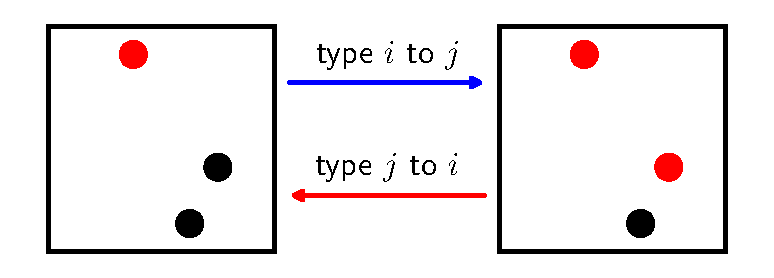
\includegraphics[width=8.5cm]{../figures/sgcmc.pdf}
\caption{
Semi-$\mu VT$ change of a particle of type $i$, shown in red, into a particle of type $j$, shown in black.
The total number of particles remains constant.
}
\label{fig:sgcmc}
\end{centering}
\end{figure}

\begin{table}
\begin{center}
\begin{tabular}{|c|c|}
 \hline
 \thead{Forward} & \thead{$\alpha_{o\rightarrow n}$} \\ [0.5ex]
 \hline
 Choose a particle of any type & $1/N_m$ \\
 \hline
 Choose new particle type $j$ & $1/(n-1)$ \\
 \hline
 Choose orientation & $P_{\omega j}\diff\boldsymbol{\omega}$ \\
 \hline
 \hline\hline
 \thead{Reverse} & \thead{$\alpha_{n\rightarrow o}$} \\ [0.5ex]
 \hline
 Choose particle of any type & $1/N_m$ \\
 \hline
 Choose new particle type $i$ & $1/(n-1)$ \\
 \hline
 Choose orientation & $P_{\omega i}\diff\boldsymbol{\omega}$ \\
 \hline
\end{tabular}
\caption{Particle type change transition probabilities.}
\label{tab:lhs_sgcmc}
\end{center}
\end{table}


Using Table~\ref{tab:lhs_sgcmc} and substituting Eq.~\ref{eq:rhs_sgcmc} into Eq.~\ref{eq:detailed_balance}, the acceptance probability for the $i\rightarrow j$ attempt as the forward transition is
\begin{equation}
\chi = \left(\frac{P_{\omega j}}{P_{\omega i}}\right)\frac{z_j}{z_i}e^{-\beta\Delta U}.
\label{eq:chisgcmc}
\end{equation}
If the particles are isotropic, or rigid and random orientations are chosen, $P_{\omega j}=P_{\omega i}$.
Otherwise, $\frac{P_{\omega j}}{P_{\omega i}}$ is related to the Rosenbluth factors for configuration bias partial regrowth or orientational bias.
Eq.~\ref{eq:chisgcmc} is tested against an $n=2$ component ideal gas mixture in Code Block~\ref{sim:ideal_gas_sgcmc}.

\begin{figure}
\lstinputlisting[
language=Python,
label={sim:ideal_gas_sgcmc},
caption={Semi-$\mu VT$ MC of a two component ideal gas mixture using Python3, and the statistics module is provided in Section~\ref{sec:block_av}.}
]{../codes/ideal_gas_sgcmc.py}
\end{figure}

%%%%%%%%%%%%%%%%%%%%%%%%%
\subsection{\label{sec:lhs_sgcmc_alt}Changing particle type by choosing a specific type}
%%%%%%%%%%%%%%%%%%%%%%%%%

In the previous Section~\ref{sec:lhs_sgcmc}, particles of multiple types are chosen randomly to attempt a change into another particle type.
Instead of choosing from all particles of any type, an alternative method is to choose one type specifically to change into another.
However, this alternative algorithm changes the acceptance criteria.

An alternative particle type change trial proceeds as follows.
First, a $i \rightarrow j$ or $j \rightarrow i$ trial is randomly chosen with equal probability.
For $i \rightarrow j$, a particle of type $i$ is randomly chosen.
A particle of type $j$ is added to the system with a fixed site in $j$ at the same position as a fixed site in $i$.
Particle $j$ is randomly oriented or regrown about its fixed site.
Particle $i$ is removed from the system.
For $j \rightarrow i$, a particle of type $j$ is randomly chosen.
A particle of type $i$ is added to the system with a fixed site in $i$ at the same position as a fixed site in $j$.
Particle $i$ is randomly oriented or regrown about its fixed site.
Particle $j$ is removed from the system.

For $i \rightarrow j$ as the forward transition, the transition probabilities are summarized in Table~\ref{tab:lhs_sgcmc_alt}, where $N_i$ and $N_j$ are the numbers of each type of particle before the trial is implemented.
Using Table~\ref{sec:lhs_sgcmc_alt} and substituting Eq.~\ref{eq:rhs_sgcmc} into Eq.~\ref{eq:detailed_balance}, the acceptance probability for the $i\rightarrow j$ attempt as the forward transition is
\begin{equation}
\chi = \frac{N_i}{N_j+1}\left(\frac{P_{\omega j}}{P_{\omega i}}\right)\frac{z_j}{z_i}e^{-\beta\Delta U}.
\label{eq:chisgcmc_alt}
\end{equation}

\begin{table}
\begin{center}
\begin{tabular}{|c|c|}
 \hline
 \thead{Forward} & \thead{$\alpha_{o\rightarrow n}$} \\ [0.5ex]
 \hline
 Choose $i \rightarrow j$ & $1/2$ \\
 \hline
 Choose particle of type $i$ & $1/N_i$ \\
 \hline
 Place $j$ on $i$ & $1$ \\
 \hline
 Choose orientation of $j$ & $P_{\omega j}\diff\boldsymbol{\omega}$ \\
 \hline
 \hline\hline
 \thead{Reverse} & \thead{$\alpha_{n\rightarrow o}$} \\ [0.5ex]
 \hline
 Choose $j \rightarrow i$ & $1/2$ \\
 \hline
 Choose particle of type $j$ & $1/(N_j+1)$ \\
 \hline
 Place $i$ on $j$ & $1$ \\
 \hline
 Choose orientation of $i$ & $P_{\omega i}\diff\boldsymbol{\omega}$ \\
 \hline
\end{tabular}
\caption{Alternative particle type change transition probabilities.}
\label{tab:lhs_sgcmc_alt}
\end{center}
\end{table}

The $j\rightarrow i$ trial is the same as Eq.~\ref{eq:chisgcmc_alt} but with $i$ and $j$ indices swapped.
If $i$ and $j$ are rigid molecules and random orientations are chosen (or if isotropic), $P_{\omega i}=P_{\omega j}$.
Otherwise, $\frac{P_{\omega j}}{P_{\omega i}}$ is related to the Rosenbluth factors for configuration bias partial regrowth.
Eq.~\ref{eq:chisgcmc_alt} is tested against an ideal gas mixture in Code Block~\ref{sim:ideal_gas_sgcmc_alt}.

\begin{figure}
\lstinputlisting[
language=Python,
label={sim:ideal_gas_sgcmc_alt},
caption={Alternative algorithm for semi-$\mu VT$ MC of an ideal gas mixture using Python3, and the statistics module is provided in Section~\ref{sec:block_av}.}
]{../codes/ideal_gas_sgcmc_alt.py}
\end{figure}

%%%%%%%%%%%%%%%%%%%%%%%%%
\section{\label{sec:rhs_gibbs}Unbiased Gibbs ensemble trials}
%%%%%%%%%%%%%%%%%%%%%%%%%

In the Gibbs ensemble, separate domains are simulated for which chemical and mechanical equilibrium at constant temperature is established between them \cite{panagiotopoulos_direct_1987}, although chemical equilibrium is sufficient to enforce mechanical equilibrium \cite{panagiotopoulos_adsorption_1987}.
For notational convenience, we will consider only two domains such that the total volume, $V=V_1+V_2$, is the sum of two volumes and the total number of particles of type $i$, $N_i$, is $N_{i1} + N_{i2}$.
Volume changes require scaling, as described in Section \ref{sec:rhs_npt}, and the particle positions must be expressed in terms of the scaled coordinates.
We do not consider constant-pressure Gibbs ensemble in this work \cite{panagiotopoulos_phase_1988}.
Although recent studies show that Gibbs (and all other) ensemble simulations may utilize a shell particle \cite{hatch_theory_2024}, we consider only the application of a shell particle in the $NPT$ ensemble in this article.

The probability of a microstate in the Gibbs ensemble is then given by \cite{panagiotopoulos_direct_1987, frenkel_understanding_2002, hatch_theory_2024},
\begin{equation}
\Pi \propto \frac{1}{\Lambda_i^{ND}}V_1^{N_{i1}}V_2^{N_{i2}} e^{-\beta (U_1+U_2)} \diff\mathbf{s}^{N} \diff V_1 \diff V_2.
\label{eq:rhs_gibbs_pi}
\end{equation}
For particle transfer between domains while holding the volume of each domain fixed, the ratio of microstates in the Gibbs ensemble with particle transfer, the first ratio of Eq.~\ref{eq:detailed_balance}, is given by
\begin{equation}
\frac{\Pi_{n}}{\Pi_{o}} = V_1^{N_{ni1}-N_{oi1}} V_2^{N_{ni2}-N_{oi2}}e^{-\beta\Delta (U_1+U_2)},
\label{eq:rhs_gibbs_particle}
\end{equation}
where $N_{ni1}$ and $N_{ni2}$ are the number of particles of type $i$ in the first and second domain, respectively, in the new microstate, while $N_{oi1}$ and $N_{oi2}$ are in the old microstate.

For volume transfer between domains while holding the number of particles in each domain fixed, the ratio of microstates in the Gibbs ensemble with volume transfer, the first ratio of Eq.~\ref{eq:detailed_balance}, is given by
\begin{equation}
\frac{\Pi_{n}}{\Pi_{o}} = \left(\frac{V_{n1}}{V_{o1}}\right)^{N_{i1}}\left(\frac{V_{n2}}{V_{o2}}\right)^{N_{i2}}e^{-\beta\Delta (U_1+U_2)},
\label{eq:rhs_gibbs_volume}
\end{equation}
where $V_{n1}$ and $V_{n2}$ are the volume of the first and second domain, respectively, in the new microstate, while $V_{o1}$ and $V_{o2}$ are in the old microstate.

%%%%%%%%%%%%%%%%%%%%%%%%%
\subsection{\label{sec:lhs_gibbs_particle}Gibbs ensemble with particle transfer trials}
%%%%%%%%%%%%%%%%%%%%%%%%%

In this example, consider particle transfers between two domains, as illustrated in Fig.~\ref{fig:gibbs_particle}.
Particle transfers are conducted similarly to a simultaneous insertion in one domain and deletion in another domain, as described in Section~\ref{sec:lhs_insdel}.
The total number of particles remains constant, as well as the volumes of both systems and the temperature.

\begin{figure}
\begin{centering}
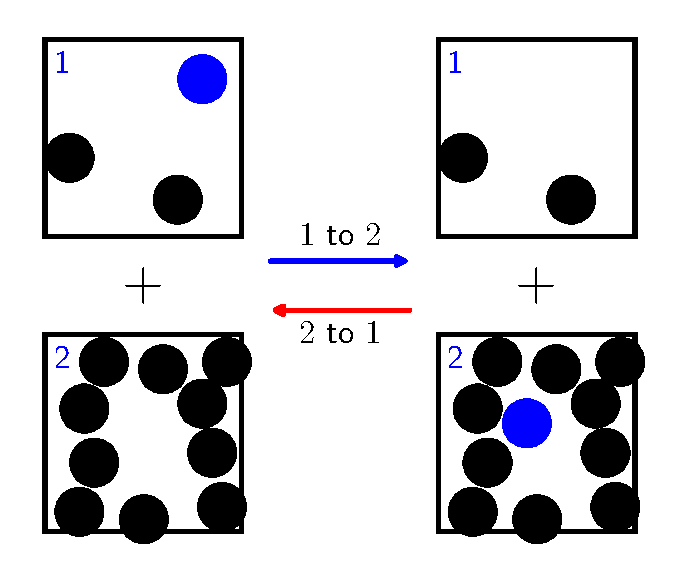
\includegraphics[width=6.5cm]{../figures/gibbs_particle.pdf}
\caption{
Gibbs ensemble transfer of the particle shown in blue from periodic domain $1$ to periodic domain $2$, and the reverse trial.
The total number of particles remains constant.
}
\label{fig:gibbs_particle}
\end{centering}
\end{figure}

Particle transfers between domains $1$ and $2$ in Gibbs ensemble MC proceed as follows.
With equal probability, domain $1$ is randomly chosen among all the domains to transfer a particle of a given type $i$.
A particle of type $i$ is then chosen for removal from domain $1$ with probability $1/N_{i1}$.
A particle of the same type is then added to domain $2$ at a random position selected uniformly within the volume, $V_2$.
The transition probabilities are summarized in Table~\ref{tab:lhs_gibbs_particle}, where $N_{i1}$ and $N_{i2}$ are the numbers of each type of particle in domains $1$ and $2$, respectively, before the trial is implemented.

\begin{table}
\begin{center}
\begin{tabular}{|c|c|}
 \hline
 \thead{Forward} & \thead{$\alpha_{o\rightarrow n}$} \\ [0.5ex]
 \hline
 Choose domain $1$ & $1/2$ \\
 \hline
 Choose particle of type $i$ in domain $1$ & $1/N_{i1}$ \\
 \hline
 Choose $\mathbf{s}_n$ in domain 2 & $\diff\mathbf{s}$ \\
 \hline
 Choose orientation of particle $i$ in domain 2 & $P_{\omega 2}\diff\boldsymbol{\omega}$ \\
 \hline\hline
 \thead{Reverse} & \thead{$\alpha_{n\rightarrow o}$} \\ [0.5ex]
 \hline
 Choose domain $2$ & $1/2$ \\
 \hline
 Choose particle of type $i$ in domain $2$ & $1/(N_{i2}+1)$ \\
 \hline
 Choose $\mathbf{s}_o$ in domain 1 & $\diff\mathbf{s}$ \\
 \hline
 Choose orientation of particle $i$ in domain 1 & $P_{\omega 1}\diff\boldsymbol{\omega}$ \\
 \hline
\end{tabular}
\caption{Gibbs ensemble particle transfer transition probabilities.}
\label{tab:lhs_gibbs_particle}
\end{center}
\end{table}

Using Table~\ref{sec:lhs_gibbs_particle} and substituting Eq.~\ref{eq:rhs_gibbs_particle} into Eq.~\ref{eq:detailed_balance}, the acceptance probability for the transfer of a particle of type $i$ from domain $1$ to domain $2$ as the forward transition is
\begin{equation}
\chi = \frac{N_{i1}}{N_{i2}+1}\left(\frac{V_2}{V_1}\right)\frac{P_{\omega 1}}{P_{\omega 2}}e^{-\beta(\Delta U_1 + \Delta U_2)}.
\label{eq:gibbs_transfer}
\end{equation}
If particles of type $i$ are rigid molecules and random orientations are chosen (or if isotropic), $P_{\omega 1}=P_{\omega 2}$.
Otherwise, $\frac{P_{\omega j}}{P_{\omega i}}$ is related to the Rosenbluth factors for configuration bias partial regrowth.
The transfer from domain $2$ to domain $1$ is identically derived by simply perturbing the indices $1$ and $2$.
Eq.~\ref{eq:gibbs_transfer} is tested in an ideal gas simulation demonstrated in Code Block~\ref{sim:gibbs_particle}, where the densities of the two domains should be equivalent \cite{hatch_theory_2024}.

\begin{figure}
\lstinputlisting[
language=Python,
label={sim:gibbs_particle},
caption={MC simulation of an ideal gas in the Gibbs ensemble with chemical equilibrium using Python3 should yield two domains with equivalent density, and the statistics module is provided in Section~\ref{sec:block_av}.}
]{../codes/ideal_gas_gibbs_particle.py}
\end{figure}

%%%%%%%%%%%%%%%%%%%%%%%%%
\subsection{\label{sec:lhs_gibbs_volume}Gibbs ensemble with volume transfer trials}
%%%%%%%%%%%%%%%%%%%%%%%%%

In this example, consider volume transfers between two domains, as illustrated in Fig.~\ref{fig:gibbs_volume}.
Volume transfers are conducted similarly to a simultaneous expansion in one domain and correlated contraction in another domain, as described in Section~\ref{sec:lhs_dv}.
The total volume, $V=V_1+V_2$, remains constant, as well as the numbers of particles of each type in both systems and the temperature.

\begin{figure}
\begin{centering}
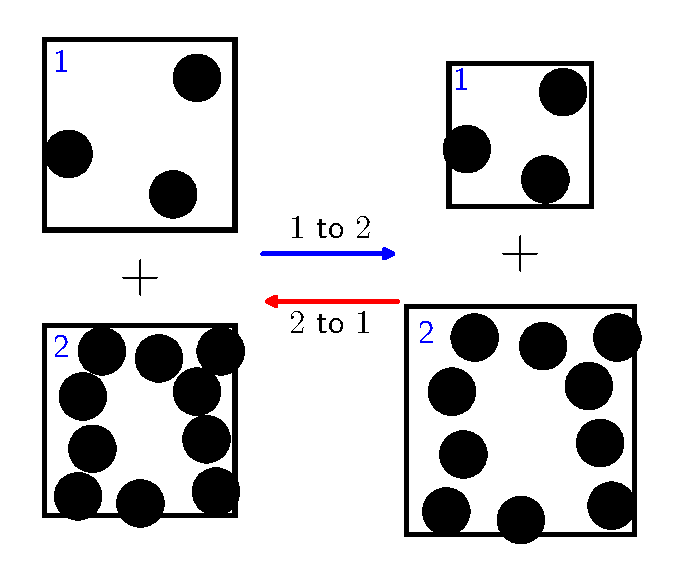
\includegraphics[width=6.5cm]{../figures/gibbs_volume.pdf}
\caption{
Gibbs ensemble transfer of volume from periodic domain $1$ to periodic domain $2$, and the reverse trial.
The total volume remains constant and the particle positions are scaled as described in Section~\ref{sec:lhs_dv}.
}
\label{fig:gibbs_volume}
\end{centering}
\end{figure}

Volume transfers between domains $1$ and $2$ in Gibbs ensemble MC proceed as follows.
As described in Section~\ref{sec:lhs_dv}, the positions of the particles and periodic boundary lengths are scaled by a factor of $(1+\Delta V/V_o)^{1/D}$ in each of $D$ dimensions, where $\Delta V$ is chosen as a random amount selected uniformly within $\pm\Delta V_{\mathrm{max}}$.
The scaling occurs with $-\Delta V$ for domain $1$, and $+\Delta V$ for domain 2, where $V_1$ and $V_2$ are the volumes of domains $1$ and $2$ before the scaling occurs.

\begin{table}
\begin{center}
% \begin{tabular}{|c|c|c|c|c|}
%  \cline{1-2}\cline{4-5}
%  \thead{Forward} & \thead{$\alpha_{o\rightarrow n}$} & & \thead{Reverse} & \thead{$\alpha_{n\rightarrow o}$}\\
%  \cline{1-2}\cline{4-5}
%  \makecell{Choose $\Delta V$} & \makecell{$\diff\mathbf{r}/(2\Delta V_{\mathrm{max}})$} & & \makecell{Choose $-\Delta V$} & \makecell{$\diff\mathbf{r}/(2\Delta V_{\mathrm{max}})$} \\
%  \cline{1-2}\cline{4-5}
\begin{tabular}{|c|c|}
 \hline
 \thead{Forward} & \thead{$\alpha_{o\rightarrow n}$} \\
 \hline
 \makecell{Choose $\Delta V$} & \makecell{$\diff\mathbf{r}/(2\Delta V_{\mathrm{max}})$} \\
 \hline\hline
 \thead{Reverse} & \thead{$\alpha_{n\rightarrow o}$}\\ [0.5ex]
 \hline
 \makecell{Choose $-\Delta V$} & \makecell{$\diff\mathbf{r}/(2\Delta V_{\mathrm{max}})$} \\
 \hline
\end{tabular}
\caption{Gibbs ensemble volume transfer transition probabilities.}
\label{tab:lhs_gibbs_volume}
\end{center}
\end{table}

Using the transition probabilities in Table~\ref{tab:lhs_gibbs_volume}, and substituting Eq.~\ref{eq:rhs_gibbs_volume} into Eq.~\ref{eq:detailed_balance}, the acceptance probability for the transfer of volume from domain $1$ to domain $2$ as the forward transition is
\begin{equation}
\chi = \left(\frac{V_1-\Delta V}{V_1}\right)^{N_{i1}} \left(\frac{V_2+\Delta V}{V_2}\right)^{N_{i2}}e^{-\beta(\Delta U_1 + \Delta U_2)}.
\label{eq:gibbs_transfer_v}
\end{equation}

Eq.~\ref{eq:gibbs_transfer_v} is tested in an ideal gas simulation demonstrated in Code Block~\ref{sim:gibbs_volume}, where the densities of the two domains should be equivalent \cite{hatch_theory_2024}.

\begin{figure}
\lstinputlisting[
language=Python,
label={sim:gibbs_volume},
caption={MC simulation of an ideal gas in the Gibbs ensemble with mechanical equilibrium using Python3 should yeild two domains with equivalent density, and the statistics module is provided in Section~\ref{sec:block_av}.}
]{../codes/ideal_gas_gibbs_volume.py}
\end{figure}

%%%%%%%%%%%%%%%%%%%%%%%%%
\subsection{\label{sec:lhs_gibbs}Gibbs ensemble with particle and volume transfer trials}
%%%%%%%%%%%%%%%%%%%%%%%%%

Gibbs ensemble simulations may include both trials with volume and particle transfers described in the previous sections.
%In this case, it is important that the shell particle cannot be transferred to another domain, and thus there should be at least one particle in each domain when the two domains are in mechanical equilibrium.
%If the two domains are not at mechanical equilibrium, as described in Section \ref{sec:lhs_gibbs_particle}, there is no need for a shell particle.
Eqs.~\ref{eq:gibbs_transfer} and \ref{eq:gibbs_transfer_v} are tested in an ideal gas simulation demonstrated in Code Block~\ref{sim:gibbs}, where the number of particles and volume should be equivalent \cite{hatch_theory_2024}.

\begin{figure}
\lstinputlisting[
language=Python,
label={sim:gibbs},
caption={MC simulation of an ideal gas in the Gibbs ensemble with mechanical and chemical equilibrium using Python3 should yield two domains with equivalent number of particles and volume.}
]{../codes/ideal_gas_gibbs.py}
\end{figure}

%%%%%%%%%%%%%%%%%%%%%%%%%
\section{\label{sec:lhs_gcmc_bias}Biased grand canonical ensemble ($\mu VT$) trials}
%%%%%%%%%%%%%%%%%%%%%%%%%

Now that all ensembles in this article have been tested with unbiased trials, we now derive biased $\mu VT$ trials.
For simulations of an ideal gas, these trials reduce to those already described in the previous sections.
Thus, ideal gas tests are not explicitly included in the remaining sections for biased trials.
However, this does not mean ideal gas tests are not useful for testing biased trials.
In fact, ideal gas tests are even more useful for biased trials where the additional complication leads to greater possibility for error.

%%%%%%%%%%%%%%%%%%%%%%%%%
\subsection{\label{sec:lhs_insdel_cb}Configurational bias (CB)}
%%%%%%%%%%%%%%%%%%%%%%%%%

In this section, we first introduce the concept of CB \cite{rosenbluth_monte_1955, siepmann_configurational_1992, mooij_direct_1992, de_pablo_estimation_1992} in an unconventional way.
In the literature, CB is typically described as a way to regrow particles with multiple interaction sites bonded together.
In this article, the orientational probabilities, $P_{\omega}$, encompass chain regrowth as well as orientational bias and anisotropic interaction sites.
The determination of $P_{\omega}$ is not discussed in detail here beyond cases where a rigid particle is randomly oriented (see Section~\ref{sec:lhs_rotation}).
Thus, we consider the application of CB only on the center of the first interaction site of a particle (e.g., multiple first bead CB).

One example of insertion and deletion of particles of type $i$ with CB proceeds as follows.
An insertion or deletion trial is randomly chosen with equal probability.
If a particle insertion is chosen, then the new position, $\mathbf{r}_n$, of a particle of type $i$ is chosen from ${c}$ random positions selected uniformly in the volume, $V$, with a relative probability of $\pi_{cn}$.
If a particle deletion is chosen, then one of $N_i$ particles of type $i$ is chosen for removal.

\begin{figure}
\begin{centering}
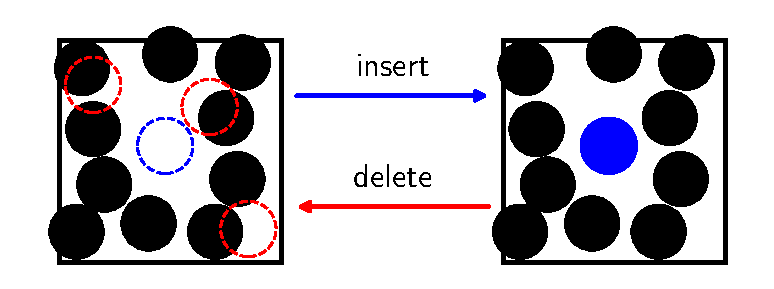
\includegraphics[width=6.5cm]{../figures/muvt_cb.pdf}
\caption{
Multiple first bead configurational bias insertion and deletion considers randomly-generated positions for a newly inserted particle, shown by the dashed circles, in an existing fluid of particles, shown by the black circles.
The most favorable position has the highest Rosenbluth probability of selection, which is shown in blue due to excluded volume overlap of the other red positions with the existing fluid.
The deletion step does not consider other positions or particles for deletion, but to obey detailed balance, the Rosenbluth factor in the deletion step includes the existing position as well as other randomly-generated positions.
}
\label{fig:muvt_cb}
\end{centering}
\end{figure}

The forward and reverse transition probabilities are summarized in Table~\ref{tab:lhs_ins_cb}.
Because the insertion is chosen as the forward transition, deletions are chosen among $N_i+1$ particles, where $N_i$ is the number of particles of type $i$ as defined from the old microstate.

\begin{table}
\begin{center}
\begin{tabular}{|c|c|}
 \hline
 \thead{Forward} & \thead{$\alpha_{o\rightarrow n}$} \\
 \hline
 Choose insert & $1/2$ \\
 \hline
 \makecell{Choose ${c}$ positions in $V$. \\ Probability that $\mathbf{r}_n$ is in ${c}$.} & ${c}\diff\mathbf{r}/V$ \\
 \hline
 Choose $\mathbf{r}_n$ from ${c}$ positions & $\pi_{cn}$ \\
 \hline
 Choose orientation & $P_{\omega n}\diff\boldsymbol{\omega}$ \\
 \hline\hline
 \thead{Reverse} & \thead{$\alpha_{n\rightarrow o}$} \\ [0.5ex]
 \hline
 Choose delete & $1/2$ \\
 \hline
 Choose particle of type $i$ & $1/(N_i + 1)$ \\
 \hline
\end{tabular}
\caption{Configurational bias particle insertion transition probabilities.}
\label{tab:lhs_ins_cb}
\end{center}
\end{table}

Using Table~\ref{tab:lhs_ins_cb} and substituting Eq.~\ref{eq:rhs_muvt} into Eq.~\ref{eq:detailed_balance}, the acceptance probability for CB particle insertion is
\begin{equation}
\chi = \frac{Vz_i}{P_{\omega n}{c}(N_i+1)\pi_{cn}}e^{-\beta\Delta U}.
\label{eq:cb_insdel}
\end{equation}

There is remarkable flexibility as to the choice of $\mathbf{r}_n$ from $c$ positions, which determines $\pi_{cn}$.
Ideally, $\pi_{cn}$ biases configurations where the energy of interaction of (the first interaction site of) a new particle at $\mathbf{r}_n$ with all the particles in the old microstate, $U_n$, is favorable.
A natural choice is to Boltzmann weight the selection of $c$ positions, $\pi_{cn} \propto e^{-\beta U_n}$.
Normalizing such a probability results in the Rosenbluth factor,
\begin{equation}
\pi_{cn} = \frac{e^{-\beta U_n}}{W_{c}},
\label{eq:rosenbluth}
\end{equation}
where
\begin{equation}
W_{c}=\sum_{i}^{c} e^{-\beta U_i}.
\label{eq:wc}
\end{equation}
Substitution of Eq.~\ref{eq:rosenbluth} into Eq.~\ref{eq:cb_insdel} yields
\begin{equation}
\chi = \frac{Vz_i W_{c}}{P_{\omega n}{c}(N_i+1)}e^{-\beta(\Delta U - U_n)}.
\label{eq:lhs_ins_cb}
\end{equation}
This form of $\pi_{cn}$ is also convenient because $\Delta U - U_n$ only contains interaction energies beyond the center of the first site (e.g., if there were multiple sites).
If there are no other orientational or multiple site interactions beyond the first bead, $\Delta U = U_n$.

The deletion step is nearly the inverse of Eq.~\ref{eq:lhs_ins_cb}, except for two details regarding the definition of $N_i$ and $\pi_{co}$.
Consider the deletion as the forward transition, where the particle is randomly chosen from $N_i$ in the old microstate.
The typical Rosenbluth factor, $W_{c}$, is calculated to satisfy detailed balance, but plays no role in the choice of the particle for deletion.
The trial with the deletion as the forward transition is described in Table~\ref{tab:lhs_del_cb}.

\begin{table}
\begin{center}
\begin{tabular}{|c|c|}
 \hline
 \thead{Forward} & \thead{$\alpha_{o\rightarrow n}$} \\ [0.5ex]
 \hline
 Choose delete & $1/2$ \\
 \hline
 Choose particle of type $i$ & $1/N_i$ \\
 \hline\hline
 \thead{Reverse} & \thead{$\alpha_{n\rightarrow o}$} \\ [0.5ex]
 \hline
 Choose insert & $1/2$ \\
 \hline
 \makecell{Choose ${c}$ positions in $V$. \\ Probability that $\mathbf{r}_o$ is in ${c}$.} & ${c}\diff\mathbf{r}/V$ \\
 \hline
 Choose $\mathbf{r}_o$ from ${c}$ positions & $\pi_{co}$ \\
 \hline
 Choose orientation & $P_{\omega o}\diff\boldsymbol{\omega}$ \\
 \hline
\end{tabular}
\caption{Configurational bias particle deletion transition probabilities.}
\label{tab:lhs_del_cb}
\end{center}
\end{table}

Thus, for deletions, the acceptance criteria using the typical Rosenbluth factor is given by,
\begin{equation}
\chi = \frac{c N_i P_{\omega o}}{Vz_i W_{c}}e^{-\beta(\Delta U + U_o)},
\label{eq:lhs_del_cb}
\end{equation}
where $\mathbf{r}_o$, the original position of the deleted particle, is among the ${c}-1$ other randomly generated positions in $\pi_{co}$, and $U_o$ is the interaction energy of the particle at $\mathbf{r}_o$ that the trial is attempting to delete.
If there are no other orientational or multiple site interactions beyond the first bead, $\Delta U = - U_o$.

In the ideal gas limit, $U\rightarrow 0$, $W_{c}\rightarrow{c}$, and Eqs.~\ref{eq:lhs_ins_cb} and \ref{eq:lhs_del_cb} are equivalent to Eqs.~\ref{eq:lhs_ins} and \ref{eq:lhs_del}.
Ideal gas simulations are helpful in quickly testing a CB implementation for verification.
Although ${c}$ in Eqs.~\ref{eq:lhs_ins_cb} and \ref{eq:lhs_del_cb} may be incorporated into the chemical potential, this may lead to confusion and is not recommended if multiple kinds of $\mu VT$ trials are attempted.

For single-site isotropic particles, such as those interacting via the Lennard-Jones potential, the orientational term (see Section~\ref{sec:lhs_rotation}) results in $P_{\omega n} = 1$ (or can be incorporated into the definition of $z_i$).
Hence, this trial is not particularly efficient compared to simply conducting $c$ traditional insertion or deletion trials sequentially.
However, this method becomes more efficient when the calculation of $P_{\omega n}$ for more complex molecules is comparable or more expensive than the calculation of $W_{c}$ (e.g., using partial regrowth or orientational bias, etc).
Another efficient approach is to use a reference potential that is less expensive than the full potential with longer-range interactions, where the reference potential still contains the most relevant terms for sampling (e.g., excluded volume in a dense fluid).
Such a method is named dual-cut CB \cite{vlugt_improving_1998} as described in the next section.

%%%%%%%%%%%%%%%%%%%%%%%%%
\subsection{\label{sec:lhs_insdel_dccb}Dual-cut configurational bias (DCCB)}
%%%%%%%%%%%%%%%%%%%%%%%%%

DCCB \cite{vlugt_improving_1998} is derived in a nearly identical fashion as CB presented in Section~\ref{sec:lhs_insdel_cb}.
The only difference is that $\pi_{cn}$ in Eq.~\ref{eq:rosenbluth} no longer uses the energy of the system, $U$, but rather, the energy of a reference system, $U_{r}$, that is, ideally, less computationally expensive to calculate.
This reference system could have a shorter cutoff distance, as per the namesake of this method.
Or, it could have a different potential or a different number of interaction sites.
For example, a simulation of SPC/E water could use a reference potential of hard spheres centered on the oxygen, which is not only short range but also reduces the number of interaction sites.
Because $\pi_{cn}$ contains the reference potential, $U_{rn}$, the insertion acceptance is given by
\begin{equation}
\chi = \frac{Vz_i W_{{c}r}}{P_{\omega nr}{c}(N_i+1)}e^{-\beta(\Delta U - U_{rn})},
\label{eq:lhs_ins_dccb}
\end{equation}
where
\begin{equation}
W_{{c}r}=\sum_{i}^{c} e^{-\beta U_{ri}}
\label{eq:wcr}
\end{equation}
and $U_{ri}$ is the reference potential contribution of the particle in microstate $i$.
Similar to Section~\ref{sec:lhs_insdel_cb}, the deletion acceptance is the inverse of the insertion, except that $N_i+1 \rightarrow N_i$, and $\mathbf{r}_o$ is one of the $c$ randomly generated positions for the calculation of $W_{{c}r}$.

The orientational term, $P_{\omega nr}$, may also utilize the reference potential, or not.
In either case, $U_{rn}$ in Eq.~\ref{eq:lhs_ins_dccb} is the sum of the (reference) interaction energies of each of the microstates chosen from both $P_{\omega nr}$ and $W_{cr}$ when the typical Rosenbluth terms are used in the probabilities of selection.

%%%%%%%%%%%%%%%%%%%%%%%%%
\subsection{\label{sec:lhs_insdel_cavity}Cavity bias}
%%%%%%%%%%%%%%%%%%%%%%%%%

Particle insertions may be biased to specific regions according to the location of cavities in a dense fluid \cite{mezei_cavity-biased_1980, mezei_grand-canonical_1987, snurr_prediction_1993, ikeda_generalization_2024}.
The practical limitation of this method is that it may become computationally expensive to identify the cavities.
In one approach, a number of test points are randomly placed in the volume for each trial \cite{mezei_cavity-biased_1980, mezei_grand-canonical_1987, snurr_prediction_1993}.
An ensemble average of the fraction of test points found within cavities, $P_c$, is then multiplied with the volume to approximate the combined volume of the cavities.
An alternative approach is to overlay the simulation domain with a discrete grid of points, as shown in Fig.~\ref{fig:cavity}.
To improve efficiency, this grid of points could be continuously updated for each trial.
In this case, the fraction of the grid that is within at least one of the cavities times the volume of the entire domain is the approximate volume of the cavities, assuming an equally spaced grid with enough resolution.
When a randomly chosen grid point within a cavity is chosen, the inserted particle may be placed at a random position selected uniformly within the voxel nearest that grid point.
In the case of an absorbent and adsorbent material, grid points that are always in the impenetrable regions of the absorbent material may be ignored \cite{snurr_prediction_1993}.
For particles with multiple sites, it may be convenient to consider just one of the sites for this cavity bias step (e.g., only the oxygen in a water molecule \cite{zhang_computational_2017}).
Voronoi tessellations may also be used to identify cavity volumes \cite{sastry_statistical_1997}.
In addition, cavity bias can also be implemented efficiently in lattice simulations \cite{barnes_structure_2009}.

\begin{figure}
\begin{centering}
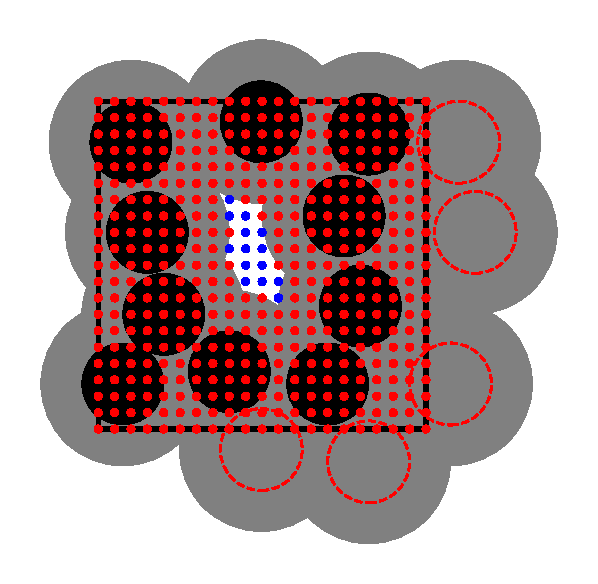
\includegraphics[width=6.5cm]{../figures/cavity.pdf}
\caption{
Cavity bias insertion and deletion may utilize a collection of points, here shown by a grid of red and blue points, which are tested for cavities.
Cavities are where another particle could fit without excluded volume overlap with existing particles, shown here as black circles with grey excluded volumes.
The red circles with dashed lines are periodic images, and the blue dots in the center are the only points in the grid that a new particle could be added onto without overlap.
}
\label{fig:cavity}
\end{centering}
\end{figure}

In this article, two variants of cavity bias will be derived.
In the first, a number of test points are chosen randomly in the domain to test for a cavity.
In the second, a predefined grid is used instead.

%%%%%%%%%%%%%%%%%%%%%%%%%
\subsubsection{\label{sec:lhs_insdel_cavity_random}Cavity bias with random test points}
%%%%%%%%%%%%%%%%%%%%%%%%%

A cavity bias trial with random test points proceeds as follows.
With equal probability, insertion or deletion of a particle of type $i$ is randomly chosen.
For insertion, $N_{test}$ points are chosen randomly in the simulation volume and $n_c$ of these points are determined to be within a cavity.
For hard particle systems, a cavity is well defined.
Soft particle systems require an ambiguous cavity definition that could affect sampling and efficiency (e.g., for the purposes of cavity determination, pick an arbitrary hard particle size for the soft particles).
Here, $n_c$ is computed for each set of randomly generated test points; the possibility of using an ensemble average of $n_c$ is discussed at the end of this section.
A particle of type $i$ is placed on one of the $n_c$ points.
For deletion, randomly choose a particle of type $i$ for removal.

With insertion as the forward transition, the transition probabilities are summarized in Table~\ref{tab:lhs_ins_cavity_random}.
Because the insertion is the forward transition, deletions are chosen among the $N_i+1$ particles, where $N_i$ is the number as defined from the old microstate.

\begin{table}
\begin{center}
\begin{tabular}{|c|c|}
 \hline
 \thead{Forward} & \thead{$\alpha_{o\rightarrow n}$} \\ [0.5ex]
 \hline
 Choose insert & $1/2$ \\
 \hline
 \makecell{Choose $N_{test}$ points in $V$.\\Probability $\mathbf{r}_n$ is in $N_{test}$.} & $N_{test}\diff\mathbf{r}/V$ \\
 \hline
 Choose $\mathbf{r}_n$ from $n_c$ & $1/n_c$ \\
 \hline
 Choose orientation & $P_{\omega n}\diff\boldsymbol{\omega}$ \\
 \hline\hline
 \thead{Reverse} & \thead{$\alpha_{n\rightarrow o}$} \\ [0.5ex]
 \hline
 Choose delete & $1/2$ \\
 \hline
 Choose particle of type $i$ & $1/(N_i+1)$ \\
 \hline
\end{tabular}
\caption{Cavity bias particle insertion transition probabilities with random test points.}
\label{tab:lhs_ins_cavity_random}
\end{center}
\end{table}

Using Table~\ref{tab:lhs_ins_cavity_random} and substituting Eq.~\ref{eq:rhs_muvt} into Eq.~\ref{eq:detailed_balance}, the acceptance probability for cavity bias particle insertion is
\begin{equation}
\chi = \left(\frac{n_c}{N_{test}}\right) \frac{z_i V}{P_{\omega n}(N_i+1)}e^{-\beta\Delta U}.
%\label{eq:dccb_insdel}
\end{equation}
For comparison to previously published articles, the probability that a random test point is in the cavity is given by $P_c = n_c/N_{test}$ \cite{mezei_cavity-biased_1980, mezei_grand-canonical_1987, snurr_prediction_1993}.
With deletion as the forward transition, the transition probabilities are summarized in Table~\ref{tab:lhs_del_cavity_random}.

\begin{table}
\begin{center}
\begin{tabular}{|c|c|}
 \hline
 \thead{Forward} & \thead{$\alpha_{o\rightarrow n}$} \\ [0.5ex]
 \hline
 Choose delete & $1/2$ \\
 \hline
 Choose particle of type $i$ & $1/N_i$ \\
 \hline\hline
 \thead{Reverse} & \thead{$\alpha_{n\rightarrow o}$} \\ [0.5ex]
 \hline
 Choose insert & $1/2$ \\
 \hline
 \makecell{Choose $N_{test}$ points in $V$.\\Probability $\mathbf{r}_o$ is in $N_{test}$.} & $N_{test}\diff\mathbf{r}/V$ \\
 \hline
 Choose $\mathbf{r}_o$ from $n_c$ & $1/n_c$ \\
 \hline
 Choose orientation & $P_{\omega o}\diff\boldsymbol{\omega}$ \\
 \hline
\end{tabular}
\caption{Cavity bias particle deletion transition probabilities with random test points.}
\label{tab:lhs_del_cavity_random}
\end{center}
\end{table}

Using Table~\ref{tab:lhs_del_cavity_random} and substituting Eq.~\ref{eq:rhs_muvt} into Eq.~\ref{eq:detailed_balance}, the acceptance probability for cavity bias particle deletions is
\begin{equation}
\chi = \frac{N_{test}}{n_c}\left(\frac{N_i P_{\omega o}}{z_i V}\right)e^{-\beta\Delta U},
\label{eq:energy_bias_del}
\end{equation}
where $n_c$ must be computed after the particle is deleted and the $N_{test}$ points includes the original position of the particle, $\mathbf{r}_o$.
For hard particle systems, a cavity is well defined and $n_c$ in the deletion step would never be zero because it includes $\mathbf{r}_o$.
But for soft interactions, depending on the definition of the cavity, $n_c$ may be zero.
If $n_c$ is zero, the trial should be rejected or else detailed balance is violated because the reverse transition is impossible.

For comparison to previously published articles \cite{mezei_cavity-biased_1980, mezei_grand-canonical_1987, snurr_prediction_1993}, it is not clear if $\mathbf{r}_o$ was included in one of the $N_{test}$ points during the deletion step.
The previous work also computed an ensemble average of $n_c$ over many trials rather than computing an instantaneous $n_c$.
An ensemble average of $n_c$ has the benefit of possibly requiring fewer $N_{test}$ points.
On the other hand, it is beyond the scope of this article to prove whether or not an ensemble average $n_c$ introduces biases via violation of detailed balance~\cite{ikeda_generalization_2024}.
The previous work also interpolated the cavity probability from other state points in special cases, and introduced unbiased insertion and deletion trials when $n_c=0$.

%%%%%%%%%%%%%%%%%%%%%%%%%
\subsubsection{\label{sec:lhs_insdel_cavity_testpoint}Cavity bias with a predefined list}
%%%%%%%%%%%%%%%%%%%%%%%%%

While Section~\ref{sec:lhs_insdel_cavity_random} used random points, a predefined list or grid, as shown in Fig.~\ref{fig:cavity}, is considered in this section.
The benefit of using a predefined list is that certain points could be removed if, for example, those grid points could never be in a cavity because of the location of a rigid wall or obstacle (e.g., an adsorbent material).
A grid is created with spacing $\delta$ in each dimension, and after points not amenable to insertion are removed, there are $N_l$ points remaining in the predefined list.

A cavity bias trial with a predefined list proceeds as follows.
With equal probability, insertion or deletion of a particle of type $i$ is randomly chosen.
For an insertion, $N_{test}$ points are randomly chosen from the fixed list of $N_l$ points, and $n_c$ of those $N_{test}$ points are determined to be within a cavity.
One of these $n_c$ points is randomly chosen, denoted as $\mathbf{r}_{nl}$.
The inserted particle of type $i$ is then placed at a random position selected uniformly within $\pm 0.5\delta$ of $\mathbf{r}_{nl}$ in each dimension.
For a deletion, randomly choose a particle of type $i$ and remove it.
In order to obey detailed balance, deletion attempts of particles that are not within $\pm 0.5\delta$ of a point in $N_l$ must be immediately rejected (e.g., if some grid points were removed yet fluid particles managed to exist in the vicinity of those removed points).
Otherwise, particles could be removed from the system where insertions could not immediately place them back for the reverse trial.

With insertion as the forward transition, the transition probabilities are summarized in Table~\ref{tab:lhs_ins_cavity_testpoint}.
Because the insertion is the forward transition, deletions are chosen among the $N_i+1$ particles, where $N_i$ is the number of particles of type $i$ as defined from the old microstate.

\begin{table}
\begin{center}
\begin{tabular}{|c|c|}
 \hline
 \thead{Forward} & \thead{$\alpha_{o\rightarrow n}$} \\ [0.5ex]
 \hline
 Choose insert & $1/2$ \\
 \hline
 \makecell{Choose $N_{test}$ points from $N_l$.\\Probability $\mathbf{r}_{nl}$ is in $N_{test}$} & $N_{test}/N_l$ \\
 \hline
 Choose $\mathbf{r}_{nl}$ from $n_c$ & $1/n_c$ \\
 \hline
 Choose $\mathbf{r}_n$ about $\mathbf{r}_{nl}$ & $\diff\mathbf{r}/\delta^D$ \\
 \hline
 Choose orientation & $P_{\omega n}\diff\boldsymbol{\omega}$ \\
 \hline\hline
 \thead{Reverse} & \thead{$\alpha_{n\rightarrow o}$} \\ [0.5ex]
 \hline
 Choose delete & $1/2$ \\
 \hline
 Choose particle of type $i$ & $1/(N_i+1)$ \\
 \hline
\end{tabular}
\caption{Cavity bias particle insertion transition probabilities with a predefined list.}
\label{tab:lhs_ins_cavity_testpoint}
\end{center}
\end{table}

Using Table~\ref{tab:lhs_ins_cavity_testpoint} and substituting Eq.~\ref{eq:rhs_muvt} into Eq.~\ref{eq:detailed_balance}, the acceptance probability for cavity bias particle insertion with $N_{test}$ points is
\begin{equation}
\chi = N_l \delta^D\left(\frac{n_c}{N_{test}}\right)\frac{z_i}{P_{\omega n}(N_i+1)}e^{-\beta\Delta U}.
\label{eq:cavity_bias_ntest}
\end{equation}
This equation takes the form of Eq.~4 of Ref.~\cite{snurr_prediction_1993} because the fraction of the points in the cavity is $P_c = n_c/N_{test}$ and the total volume considered for insertions is $v=N_l\delta^D$.

With deletion as the forward transition, the position of the chosen particle to be deleted is $\mathbf{r}_o$, which is within $\delta$ in each dimension of a point within the predefined list, $\mathbf{r}_{ol}$.
If not, the deletion is rejected to obey detailed balance.
The transition probabilities are summarized in Table~\ref{tab:lhs_del_cavity_testpoint}.

\begin{table}
\begin{center}
\begin{tabular}{|c|c|}
 \hline
 \thead{Forward} & \thead{$\alpha_{o\rightarrow n}$} \\ [0.5ex]
 \hline
 Choose delete & $1/2$ \\
 \hline
 Choose particle of type $i$ & $1/N_i$ \\
 \hline\hline
 \thead{Reverse} & \thead{$\alpha_{n\rightarrow o}$} \\ [0.5ex]
 \hline
 Choose insert & $1/2$ \\
 \hline
 \makecell{Choose $N_{test}$ from $N_l$ points.\\Probability $\mathbf{r}_{ol}$ is in $N_{test}$} & $N_{test}/N_l$ \\
 \hline
 Choose $\mathbf{r}_{ol}$ from $n_c$ & $1/n_c$ \\
 \hline
 Choose $\mathbf{r}_o$ about $\mathbf{r}_{ol}$ & $\diff\mathbf{r}/\delta^D$ \\
 \hline
 Choose orientation & $P_{\omega o}\diff\boldsymbol{\omega}$ \\
 \hline
\end{tabular}
\caption{Cavity bias particle deletion transition probabilities with a predefined list.}
\label{tab:lhs_del_cavity_testpoint}
\end{center}
\end{table}

Using Table~\ref{tab:lhs_del_cavity_testpoint} and substituting Eq.~\ref{eq:rhs_muvt} into Eq.~\ref{eq:detailed_balance}, the acceptance probability for cavity bias particle deletions with $N_{test}$ points is
\begin{equation}
\chi = \frac{1}{N_l \delta^D}\left(\frac{N_{test}}{n_c}\right)\frac{N_i P_{\omega o}}{z_i}e^{-\beta\Delta U}.
\label{eq:cavity_bias_ntest_del}
\end{equation}
Similar to Eq.~\ref{eq:energy_bias_del}, $n_c$ is computed after the particle is deleted and includes $\mathbf{r}_{ol}$, which is the closest grid point to the old macrostate position of the deleted particle, $\mathbf{r}_o$.

%%%%%%%%%%%%%%%%%%%%%%%%%
\subsection{\label{sec:lhs_insdel_energybias}Energy bias}
%%%%%%%%%%%%%%%%%%%%%%%%%

Particle insertions may also be biased in specific regions according to their energy of interaction with a fixed adsorbent material \cite{snurr_prediction_1993}, as illustrated in Fig.~\ref{fig:energybias}.
The simulation volume is divided into a number of small voxels with volume $v$.
Energy bias particle insertions and deletions proceed as follows.
With equal probability, an insertion or deletion is attempted.
For an insertion, a voxel is randomly chosen with probability $P_c$.
A new particle of type $i$ is then randomly placed inside of the chosen voxel.
For a deletion, an existing particle of type $i$ is chosen randomly and removed from the system.
The trial probabilities are summarized with insertion as the forward transition in Table~\ref{tab:lhs_ins_energybias}.

\begin{figure}
\begin{centering}
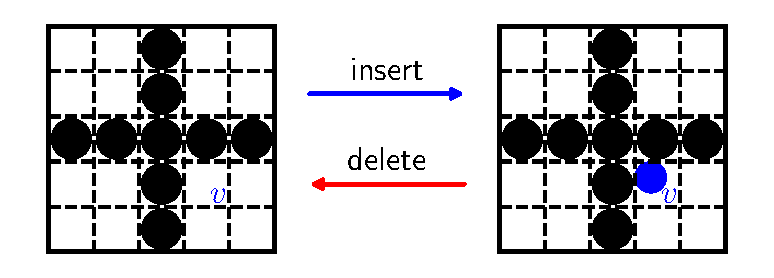
\includegraphics[width=6.5cm]{../figures/energybias.pdf}
\caption{
Energy bias insertion and deletion \cite{snurr_prediction_1993} divides the simulation domain into voxels, with $25$ shown here by the dashed lines.
One voxel, $v$, is chosen for the available insertion volume according to a probability Boltzmann-weighted by the energy of interaction with a rigid adsorbent frame, shown by the black circles.
The reverse move is when the newly inserted fluid particle, shown in blue, is randomly chosen for deletion among all the fluid particles.
}
\label{fig:energybias}
\end{centering}
\end{figure}

\begin{table}
\begin{center}
\begin{tabular}{|c|c|}
 \hline
 \thead{Forward} & \thead{$\alpha_{o\rightarrow n}$} \\ [0.5ex]
 \hline
 Choose insert & $1/2$ \\
 \hline
 Choose voxel & $P_c$ \\
 \hline
 Choose position in $v$ & $\diff\mathbf{r}/v$ \\
 \hline
 Choose orientation & $P_{\omega n}\diff\boldsymbol{\omega}$ \\
 \hline\hline
 \thead{Reverse} & \thead{$\alpha_{n\rightarrow o}$} \\ [0.5ex]
 \hline
 Choose delete & $1/2$ \\
 \hline
 Choose particle of type $i$ & $1/(N_i+1)$ \\
 \hline
\end{tabular}
\caption{Energy bias particle insertion transition probabilities.}
\label{tab:lhs_ins_energybias}
\end{center}
\end{table}

Substituting Eq.~\ref{eq:rhs_muvt} into the first ratio in Eq.~\ref{eq:detailed_balance}, and using Table~\ref{tab:lhs_ins_energybias} for the second ratio in Eq.~\ref{eq:detailed_balance}, results in
\begin{equation}
\chi = \frac{v z_i}{P_{\omega n}(N_i+1)P_c} e^{-\beta\Delta U}
\label{eq:lhs_ins_energybias}
\end{equation}
for energy bias insertions.
Deletions as the forward trial is summarized in Table~\ref{tab:lhs_del_energybias}.

\begin{table}
\begin{center}
\begin{tabular}{|c|c|}
 \hline
 \thead{Forward} & \thead{$\alpha_{o\rightarrow n}$} \\ [0.5ex]
 \hline
 Choose delete & $1/2$ \\
 \hline
 Choose particle of type $i$ & $1/N_i$ \\
 \hline\hline
 \thead{Reverse} & \thead{$\alpha_{n\rightarrow o}$} \\ [0.5ex]
 \hline
 Choose insert & $1/2$ \\
 \hline
 Choose voxel & $P_c$ \\
 \hline
 Choose position in $v$ & $\diff\mathbf{r}/v$ \\
 \hline
 Choose orientation & $P_{\omega o}\diff\boldsymbol{\omega}$ \\
 \hline
\end{tabular}
\caption{Energy bias particle deletion transition probabilities.}
\label{tab:lhs_del_energybias}
\end{center}
\end{table}

Substituting Eq.~\ref{eq:rhs_muvt} into the first ratio in Eq.~\ref{eq:detailed_balance}, and using Table~\ref{tab:lhs_del_energybias} for the second ratio in Eq.~\ref{eq:detailed_balance}, results in
\begin{equation}
\chi = \frac{N_i P_c P_{\omega o}}{v z_i} e^{-\beta\Delta U}
\label{eq:lhs_del_energybias}
\end{equation}
for deletions as the reverse of energy bias insertions.

For both insertions and deletions, a suitable $P_c$ must be utilized that is ideally inexpensive to compute and increases sampling in the desired location.
As originally formulated, a good choice for $P_c$ is to weight the probability by the Boltzmann factor of the energy a particle in the center of the chosen target volume, $v$, would have with an adsorbent material, $U^a_t$,
\begin{equation}
P_c = \frac{e^{-\beta U^a_t}}{\sum_i e^{-\beta U^a_i}}.
\label{eq:lhs_energybias_pt}
\end{equation}

%%%%%%%%%%%%%%%%%%%%%%%%%
\subsection{\label{sec:lhs_insdel_subset}Insertion and deletion in a targeted region}
%%%%%%%%%%%%%%%%%%%%%%%%%

Particle insertions and deletions may also be performed in a targeted region, $v$, shown in Fig.~\ref{fig:muvt_target} with a rigid adsorbent framework.
The trial proceeds as follows.
First, a particle insertion or deletion trial is chosen randomly with equal probability.
If a particle insertion trial is chosen, then a particle of type $i$ is placed at a random position selected uniformly in a targeted region, $v$, with random orientation.
If a particle deletion trial is chosen, then a random particle of type $i$ within $v$ is chosen for removal.
Here, $n_i$ is the number of particles of type $i$ inside $v$ at the beginning of the trial.
For particle deletions, if $n_i=0$, then reject the trial.
To obey detailed balance, $v$ cannot change during the trial.
The transition probability of an insertion trial as the forward transition is then summarized in Table~\ref{tab:lhs_ins_subset}.

\begin{figure}
\begin{centering}
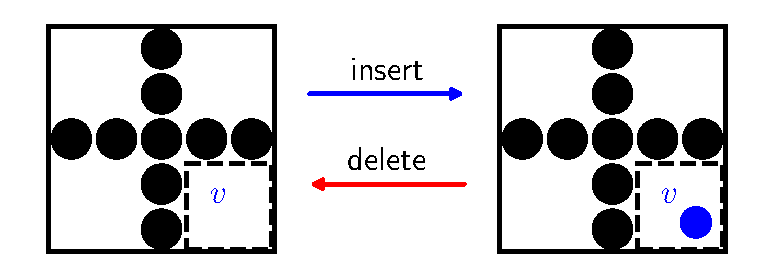
\includegraphics[width=6.5cm]{../figures/muvt_target.pdf}
\caption{
Insertion and deletion trials in a targeted region, $v$.
Similar to Fig.~\ref{fig:energybias}, the targeted region could be carefully chosen to avoid excluded volume overlap with a rigid adsorbent framework.
}
\label{fig:muvt_target}
\end{centering}
\end{figure}

\begin{table}
\begin{center}
\begin{tabular}{|c|c|}
 \hline
 \thead{Forward} & \thead{$\alpha_{o\rightarrow n}$} \\ [0.5ex]
 \hline
 Choose insert & $1/2$ \\
 \hline
 Choose position in $v$ & $\diff\mathbf{r}/v$ \\
 \hline
 Choose orientation & $P_{\omega n}\diff\boldsymbol{\omega}$ \\
 \hline\hline
 \thead{Reverse} & \thead{$\alpha_{n\rightarrow o}$} \\ [0.5ex]
 \hline
 Choose delete & $1/2$ \\
 \hline
 Choose particle of type $i$ in $v$ & $1/(n_i+1)$ \\
 \hline
\end{tabular}
\caption{Particle insertion transition probabilities in a targeted region.}
\label{tab:lhs_ins_subset}
\end{center}
\end{table}

Substituting Eq.~\ref{eq:rhs_muvt} into the first ratio in Eq.~\ref{eq:detailed_balance}, and using Table~\ref{tab:lhs_ins_subset} for the second ratio in Eq.~\ref{eq:detailed_balance}, results in
\begin{equation}
\chi = \frac{v z_i}{P_{\omega n}(n_i+1)} e^{-\beta\Delta U},
\label{eq:lhs_ins_target}
\end{equation}
where $n_i$ is defined as the number of particles of type $i$ inside $v$ at the beginning of the insertion trial (i.e., before insertion).
The transition probability of a deletion trial as the forward transition is then summarized in Table~\ref{tab:lhs_del_subset}.

\begin{table}
\begin{center}
\begin{tabular}{|c|c|}
 \hline
 \thead{Forward} & \thead{$\alpha_{o\rightarrow n}$} \\ [0.5ex]
 \hline
 Choose delete & $1/2$ \\
 \hline
 Choose particle of type $i$ in $v$ & $1/n_i$ \\
 \hline\hline
 \thead{Reverse} & \thead{$\alpha_{n\rightarrow o}$} \\ [0.5ex]
 \hline
 Choose insert & $1/2$ \\
 \hline
 Choose position in $v$ & $\diff\mathbf{r}/v$ \\
 \hline
 Choose orientation & $P_{\omega o}\diff\boldsymbol{\omega}$ \\
 \hline
\end{tabular}
\caption{Particle deletion transition probabilities in a targeted region.}
\label{tab:lhs_del_subset}
\end{center}
\end{table}

Substituting Eq.~\ref{eq:rhs_muvt} into the first ratio in Eq.~\ref{eq:detailed_balance}, and using Table~\ref{tab:lhs_del_subset} for the second ratio in Eq.~\ref{eq:detailed_balance}, results in
\begin{equation}
\chi = \frac{n_i P_{\omega o}}{v z_i} e^{-\beta\Delta U},
\label{eq:lhs_del_target}
\end{equation}
where $n_i$ is defined as the number of particles of type $i$ inside $v$ at the beginning of the deletion trial (i.e., before deletion).

%%%%%%%%%%%%%%%%%%%%%%%%%
\subsection{\label{sec:lhs_insdel_avb}Aggregation volume bias (AVB)}
%%%%%%%%%%%%%%%%%%%%%%%%%

\begin{figure}
\begin{centering}
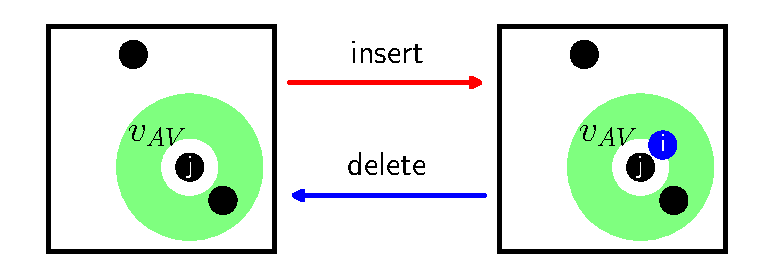
\includegraphics[width=6.5cm]{../figures/avb.pdf}
\caption{
Insertion and deletion of a blue particle of type $i$ within the aggregation volume (AV), shown in green, of an existing particle of type $j$.
}
\label{fig:avb_gce}
\end{centering}
\end{figure}

AVB insertions and deletions specifically target the positions near other molecules \cite{chen_improving_2001} in order to improve sampling for aggregated clusters of molecules, as shown in Fig.~\ref{fig:avb_gce}.
In these derivations, aggregation volumes (AVs) are defined uniquely by one specific interaction site on a target particle and one specific site on a mobile particle.
A single site should be specifically defined, not a type of site when there are multiple sites of the same type, or else detailed balance may be broken.
Instead, if multiple AVs are desired in a single target particle, then simply treat each as a separate trial.
For an isotropic AV, the mobile particle is inside the AV of the target particle if the distance between the two sites is between $r_{inner}$ and $r_{outer}$.

An attempted AVB insertion and deletion proceeds as follows.
First, an insertion or deletion trial is chosen randomly with equal probability.
If a particle insertion is chosen, then the new position, $\mathbf{r}_n$, of an interaction site of the new particle of type $i$ is placed at a random position selected uniformly within the AV, $v_{AV}$, of a different particle of type $j$ that is randomly chosen from among $N_j$ particles.
The AV, in this example, is defined using the spherical shell between $r_{inner}$ and $r_{outer}$, although it is possible to define an orientation-specific AV \cite{rovigatti_how_2018}.
See Section~\ref{sec:spherical_shell} for how to generate randomly uniform points in a spherical shell.
The remaining sites in the new particle may be oriented randomly about $\mathbf{r}_n$ or regrown with CB.
If a particle deletion is chosen, then a particle of type $j$ is randomly chosen.
A random particle of type $i$ within the AV of the chosen particle of type $j$ is removed from among the $N_i^{AV}$ particles of type $i$ within the AV.
The transition probabilities with insertion as the forward transition is summarized in Table~\ref{tab:lhs_ins_avb}.

\begin{table}
\begin{center}
\begin{tabular}{|c|c|}
 \hline
 \thead{Forward} & \thead{$\alpha_{o\rightarrow n}$} \\ [0.5ex]
 \hline
 Choose insert & $1/2$ \\
 \hline
 Choose particle of type $j$ & $1/N_j$ \\
 \hline
 Choose $\mathbf{r}_n$ in AV & $\diff\mathbf{r}/v_{AV}$ \\
 \hline
 Choose orientation & $P_{\omega n}\diff\boldsymbol{\omega}$ \\
 \hline\hline
 \thead{Reverse} & \thead{$\alpha_{n\rightarrow o}$} \\ [0.5ex]
 \hline
 Choose delete & $1/2$ \\
 \hline
 Choose particle of type $j$ & $1/(N_j + \delta_{ij})$ \\
 \hline
 Choose interaction site in AV& $1/(N_i^{AV} + 1)$ \\
 \hline
\end{tabular}
\caption{AVB particle insertion transition probabilities.}
\label{tab:lhs_ins_avb}
\end{center}
\end{table}

If particle type $i$ and $j$ are identical, then $\delta_{ij}=1$.
Otherwise, $\delta_{ij}=0$.
Substituting Eq.~\ref{eq:rhs_muvt} into the first ratio in Eq.~\ref{eq:detailed_balance}, and using Table~\ref{tab:lhs_ins_avb} for the second ratio in Eq.~\ref{eq:detailed_balance}, results in
\begin{equation}
\chi = \frac{N_j}{N_j+\delta_{ij}}\left[\frac{v_{AV}z_i}{P_{\omega n}(N_i^{AV}+1)}\right] e^{-\beta\Delta U}.
\label{eq:lhs_gc_avb_add}
\end{equation}

Deletions are derived in an identical fashion, except that $N^{AV}_i$ is evaluated from the perspective of the state before the deletion (e.g., after insertions), and the trial is summarized in Table~\ref{tab:lhs_del_avb}.
The deletion acceptance is obtained by substituting Eq.~\ref{eq:rhs_muvt} into the first ratio in Eq.~\ref{eq:detailed_balance}, and using Table~\ref{tab:lhs_del_avb} for the second ratio in Eq.~\ref{eq:detailed_balance}, resulting in
\begin{equation}
\chi = \frac{N_j}{N_j-\delta_{ij}}\left(\frac{N^{AV}_i P_{\omega o}}{v_{AV}z_i}\right)e^{-\beta\Delta U}.
\label{eq:lhs_gc_avb_del}
\end{equation}

\begin{table}
\begin{center}
\begin{tabular}{|c|c|}
 \hline
 \thead{Forward} & \thead{$\alpha_{o\rightarrow n}$} \\ [0.5ex]
 \hline
 Choose delete & $1/2$ \\
 \hline
 Choose particle of type $j$ & $1/N_j$ \\
 \hline
 Choose interaction site in AV& $1/N_i^{AV}$ \\
 \hline\hline
 \thead{Reverse} & \thead{$\alpha_{n\rightarrow o}$} \\ [0.5ex]
 \hline
 Choose insert & $1/2$ \\
 \hline
 Choose particle of type $j$ & $1/(N_j - \delta_{ij})$ \\
 \hline
 Choose $\mathbf{r}_o$ in AV & $\diff\mathbf{r}/v_{AV}$ \\
 \hline
 Choose orientation & $P_{\omega o}\diff\boldsymbol{\omega}$ \\
 \hline
\end{tabular}
\caption{AVB particle deletion transition probabilities.}
\label{tab:lhs_del_avb}
\end{center}
\end{table}

%%%%%%%%%%%%%%%%%%%%%%%%%
\section{\label{sec:lhs_nvt_bias}Biased canonical ensemble ($NVT$) trials}
%%%%%%%%%%%%%%%%%%%%%%%%%


In this section, biased $NVT$ trials are derived.
First, we consider AVB displacement trials.
Displacement trials include both linear and angular displacement.
There are a few variants of AVB to consider.
Although inefficiencies were found in the original version \cite{chen_aggregation-volume-bias_2001, wierzchowski_general-purpose_2001, wierzchowski_ub_2002}, the second variant, AVBMC2, efficiently moves particles in and out of the AV \cite{chen_improving_2001}.
A third variant, AVBMC3, allows for particles to move from the AV of one particle into the AV of another particle (denoted as ``in $\rightarrow$ in") \cite{chen_improving_2001}.
First, we introduce AVBMC2.
Then, we derive the ``in $\rightarrow$ in" part of AVBMC3, and then introduce a relatively new variant of AVBMC3 that we call AVBMC4 \cite{siderius_flat-histogram_2024}, which is very similar to AVBMC3 but allows for overlapping AVs.
After AVB, we also derive CB and DCCB displacements in the $NVT$ ensemble.

%%%%%%%%%%%%%%%%%%%%%%%%%
\subsection{\label{sec:lhs_disp_avb2}Displacement with aggregation volume bias (AVBMC2)}
%%%%%%%%%%%%%%%%%%%%%%%%%

\begin{figure}
\begin{centering}
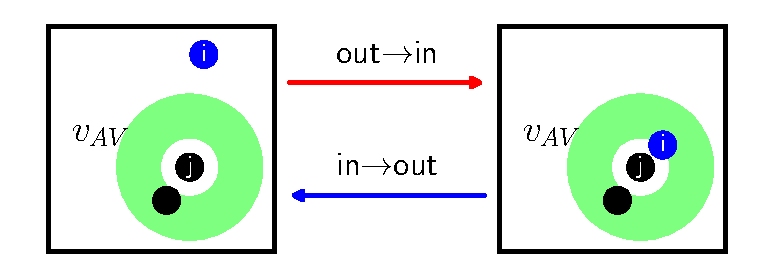
\includegraphics[width=6.5cm]{../figures/avb2.pdf}
\caption{
AVBMC2 displacement of a blue particle of type $i$ from outside to inside the AV, $v_{AV}$ shown in green, of an existing target particle of type $j$, and the reverse trial.
}
\label{fig:avbmc2}
\end{centering}
\end{figure}

In AVBMC2, a target particle of type $j$ is chosen randomly from $N_j$ particles.
The AV is then defined about one specific site in the target particle.
The mobile particle with one specific site then attempts a move into or out of the AV, with $N_i$ particles of this type.
The target and mobile particles may be the same.
In this case, $\delta_{ij}=1$, otherwise, $\delta_{ij}=0$.
At the beginning of the trial, there are $N_i^{AV}$ particles of type $i$ inside the AV of the specific site in the chosen particle of type $j$.
AVBMC2 is an $NVT$ trial because the total number of particles does not change.

In the AVB algorithm, it is possible for a particle to be inserted into an AV such that it happens to fall in the AV of two other particles, so that there would be more than one way to transition to the same microstate.
The transition probabilities do not need to account for this circumstance, because super-detailed balance is satisfied for each path.
The unbonding bonding (UB) algorithm \cite{wierzchowski_general-purpose_2001} presents a variation of the AVB algorithm that more explicitly accounts for these cases.

The AVBMC2 trial proceeds as follows.
A target particle of type $j$ is chosen randomly from $N_j$ and the AV is defined about the specific site in the chosen particle.
With probability $P_{bias}$, an ``out $\rightarrow$ in" trial is performed.
Otherwise, an ``in $\rightarrow$ out" trial is performed.
For ``out $\rightarrow$ in," one of $N_i$ particles of type $i$ is chosen randomly that has the specific site in $i$ that is not in the AV.
The chosen mobile site of the particle of type $i$ is then placed at a random position selected uniformly in the AV.
If the particle has other sites, they may then be regrown with CB or randomly rotated.
For ``in $\rightarrow$ out," one of the $N_i^{AV}$ sites in the AV is placed randomly in the entire simulation domain that is not in the AV.
Again, the remainder of the particle may then be oriented randomly or regrown with CB.

The transition probabilities for AVBMC2 are summarized in Table~\ref{tab:lhs_disp_in_avb2} for a forward transition of ``out $\rightarrow$ in."
The reverse move always has $N_i^{AV}+1$ in the AV, where $N_i^{AV}$ is the number of mobile sites in particles of type $m$ in the AV at the beginning of the trial.

\begin{table}
\begin{center}
\begin{tabular}{|c|c|}
 \hline
 \thead{Forward} & \thead{$\alpha_{o\rightarrow n}$} \\ [0.5ex]
 \hline
 Choose particle of type $j$ & $1/N_j$ \\
 \hline
 Choose ``out $\rightarrow$ in" & $P_{bias}$ \\
 \hline
 Choose mobile site not in AV & $1/(N_i - N_i^{AV} - \delta_{ij})$ \\
 \hline
 Choose $\mathbf{r}_n$ in AV & $\diff\mathbf{r}/v_{AV}$ \\
 \hline
 Choose orientation & $P_{\omega n}\diff\boldsymbol{\omega}$ \\
 \hline\hline
 \thead{Reverse} & \thead{$\alpha_{n\rightarrow o}$} \\ [0.5ex]
 \hline
 Choose particle of type $j$ & $1/N_j$ \\
 \hline
 Choose ``in $\rightarrow$ out" & $1-P_{bias}$ \\
 \hline
 Choose mobile site in AV & $1/(N_i^{AV} + 1)$ \\
 \hline
 Choose $\mathbf{r}_o$ outside AV & $\diff\mathbf{r}/(V - v_{AV})$ \\
 \hline
 Choose orientation & $P_{\omega o}\diff\boldsymbol{\omega}$ \\
 \hline
\end{tabular}
\caption{Particle displacement AVBMC2 ``out $\rightarrow$ in" transition probabilities.}
\label{tab:lhs_disp_in_avb2}
\end{center}
\end{table}

Using Table~\ref{tab:lhs_disp_in_avb2} and substituting Eq.~\ref{eq:rhs_nvt} into Eq.~\ref{eq:detailed_balance}, the acceptance probability is
\begin{equation}
\chi = \frac{P_{\omega o}(1-P_{bias})(N_i-N_i^{AV}-\delta_{ij})v_{AV}}{P_{\omega n} P_{bias}(N_i^{AV}+1)(V-v_{AV})}e^{-\beta \Delta U}.
\label{eq:avb2outin}
\end{equation}
For an example of combining AVB with CB, see the Appendix of Ref.~\cite{hatch_self-assembly_2016}.

The transition probabilities for ``in $\rightarrow$ out" as the forward transition are summarized in Table~\ref{tab:lhs_disp_out_avb2}.
Using Table~\ref{tab:lhs_disp_out_avb2} and substituting Eq.~\ref{eq:rhs_nvt} into Eq.~\ref{eq:detailed_balance}, the acceptance probability is
\begin{equation}
\chi = \frac{P_{\omega o} P_{bias}N_i^{AV}(V/v_{AV}-1)e^{-\beta \Delta U}}{P_{\omega n}(1-P_{bias})(N_i-N_i^{AV}-\delta_{ij}+1)}.
\label{eq:avb2inout}
\end{equation}

\begin{table}
\begin{center}
\begin{tabular}{|c|c|}
 \hline
 \thead{Forward} & \thead{$\alpha_{o\rightarrow n}$} \\ [0.5ex]
 \hline
 Choose particle of type $j$ & $1/N_j$ \\
 \hline
 Choose ``in $\rightarrow$ out" & $1-P_{bias}$ \\
 \hline
 Choose mobile site in AV & $1/N_i^{AV}$ \\
 \hline
 Choose $\mathbf{r}_n$ outside AV & $\diff\mathbf{r}/(V - v_{AV})$ \\
 \hline
 Choose orientation & $P_{\omega n}\diff\boldsymbol{\omega}$ \\
 \hline\hline
 \thead{Reverse} & \thead{$\alpha_{n\rightarrow o}$} \\ [0.5ex]
 \hline
 Choose particle of type $j$ & $1/N_j$ \\
 \hline
 Choose ``out $\rightarrow$ in" & $P_{bias}$ \\
 \hline
 Choose mobile site not in AV & $1/(N_i - N_i^{AV} - \delta_{ij} + 1)$ \\
 \hline
 Choose $\mathbf{r}_o$ in AV & $\diff\mathbf{r}/v_{AV}$ \\
 \hline
 Choose orientation & $P_{\omega o}\diff\boldsymbol{\omega}$ \\
 \hline
\end{tabular}
\caption{Particle displacement AVBMC2 ``in $\rightarrow$ out" transition probabilities.}
\label{tab:lhs_disp_out_avb2}
\end{center}
\end{table}

%%%%%%%%%%%%%%%%%%%%%%%%%
\subsection{\label{sec:lhs_disp_avb34}Displacement from one aggregation volume to another (AVBMC3/4)}
%%%%%%%%%%%%%%%%%%%%%%%%%

\begin{figure}
\begin{centering}
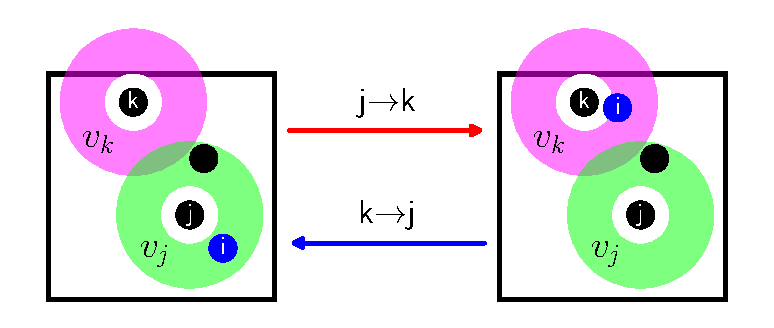
\includegraphics[width=6.5cm]{../figures/avb4.pdf}
\caption{
AVBMC4 displacement of a blue particle of type $m$ from inside the AV, $v_j$ of an existing target particle of type $j$, into the AV of an existing target particle $k$, $v_k$, and the reverse trial.
AVBMC3 does not allow overlapping AV as shown here \cite{chen_improving_2001}.
}
\label{fig:avbmc4}
\end{centering}
\end{figure}

In addition to moves inside and outside of AVs, such as AVBMC2 as described in Section~\ref{sec:lhs_disp_avb2}, moves from one AV to another are also possible, as done in AVBMC3 \cite{chen_improving_2001}.
In this case, two target particles are randomly chosen, and a third mobile particle is moved from the AV of the first target into the AV of the second target.
In the original formulation, AVBMC2 type moves were also considered.
To simplify the acceptance criteria, the AV of the two target particles also could not overlap.
In this section, we describe a variation of AVBMC3, here called AVBMC4 \cite{siderius_flat-histogram_2024}, with two subtle differences from AVBMC3.
First, AVBMC4 does not contain AVBMC2 ``in $\rightarrow$ out" or "out $\rightarrow$ in" moves.
Second, AVBMC4 allows the AV of the target particles to overlap, as long as the two target particles are not inside the AV of the other.

The AVBMC4 trial proceeds as follows.
Two target particles are chosen randomly from all particles of type $j$ and $k$, respectively.
If types $j$ and $k$ are the same, then $\delta_{jk}=1$ and particle $k$ is chosen randomly from $N_k-1$ particles because it cannot be the identical particle $j$.
The AV of the $j$ particle, $v_j$, is defined about one specific site in the $j$ particle.
Similarly, the AV of the $k$ particle, $v_k$, is defined about a specific site in the $k$ particle.
Choose a $k\rightarrow j$ attempt with probability $P_{bias}$, otherwise attempt a $j\rightarrow k$ trial.
For a $j\rightarrow k$ attempt, a mobile particle of type $i$ that has a specific site inside $v_j$, but is not the same particle as the first two chosen $j$ and $k$ particles, is then moved inside $v_k$.
If the $i$ particle has multiple sites or orientation, then it should be randomly oriented or randomly regrown with CB.
For a $k\rightarrow j$ attempt, a mobile particle of type $i$ that has a specific site inside $v_k$, but is not the same particle as the first two chosen $j$ and $k$ particles, is then moved inside $v_j$.

Because $v_j$ and $v_k$ may overlap in AVBMC4, there are a few extra caveats to consider.
If the interaction site in particle $i$ is already inside $v_k$ at the beginning of the trial, then $\Delta_{ik}=1$ and there are $N_i^{in,k} - \Delta_{ik} + 1$ available sites to choose the mobile particle in the reverse move from $v_k$ to $v_j$.
Furthermore, the two targets, $j$ and $k$, cannot be inside the AV of each other, or the trial is rejected.
This trial is summarized in Table~\ref{tab:lhs_disp_avb34}.

\begin{table}
\begin{center}
\begin{tabular}{|c|c|}
 \hline
 \thead{Forward} & \thead{$\alpha_{o\rightarrow n}$} \\ [0.5ex]
 \hline
 Choose $j\rightarrow k$ & $1-P_{bias}$ \\
 \hline
 Choose particle of type $j$ & $1/N_j$ \\
 \hline
 Choose particle of type $k$ & $1/(N_k-\delta_{jk})$ \\
 \hline
 Choose mobile site in $v_j$ & $1/N_i^{in,j}$ \\
 \hline
 Choose $\mathbf{r}_n$ in $v_k$ & $\diff\mathbf{r}/v_k$ \\
 \hline
 Choose orientation & $P_{\omega n}\diff\boldsymbol{\omega}$ \\
 \hline\hline
 \thead{Reverse} & \thead{$\alpha_{n\rightarrow o}$} \\ [0.5ex]
 \hline
 Choose $k\rightarrow j$ & $P_{bias}$ \\
 \hline
 Choose particle of type $j$ & $1/N_j$ \\
 \hline
 Choose particle of type $k$ & $1/(N_k-\delta_{jk})$ \\
 \hline
 Choose mobile site in $v_k$ & $1/(N_i^{in,k} - \Delta_{ik} + 1)$ \\
 \hline
 Choose $\mathbf{r}_o$ in $v_j$ & $\diff\mathbf{r}/v_j$ \\
 \hline
 Choose orientation & $P_{\omega o}\diff\boldsymbol{\omega}$ \\
 \hline
\end{tabular}
\caption{Particle displacement from one AV to another (AVBMC3/4) transition probabilities.}
\label{tab:lhs_disp_avb34}
\end{center}
\end{table}

Using Table~\ref{tab:lhs_disp_avb34} and substituting Eq.~\ref{eq:rhs_nvt} into Eq.~\ref{eq:detailed_balance}, the acceptance probability for the $j\rightarrow k$ attempt as the forward transition is
\begin{equation}
\chi = \frac{P_{bias}}{1-P_{bias}}\left(\frac{v_k P_{\omega o}}{v_j P_{\omega n}}\right)\frac{N_i^{in,j}}{N_i^{in,k} - \Delta_{ik} + 1}e^{-\beta \Delta U}.
\label{eq:avb4jk}
\end{equation}

The acceptance probability for the $k\rightarrow j$ attempt as the forward transition is obtained by perturbing the $j$ and $k$ in Eq.~\ref{eq:avb4jk} and inverting the $P_{bias}$ term to yield
\begin{equation}
\chi = \frac{1-P_{bias}}{P_{bias}}\left(\frac{v_j P_{\omega o}}{v_k P_{\omega n}}\right)\frac{N_i^{in,k}}{N_i^{in,j} - \Delta_{ij} + 1}e^{-\beta \Delta U}.
\label{eq:avb3inin}
\end{equation}


%%%%%%%%%%%%%%%%%%%%%%%%%
\subsection{\label{sec:lhs_disp_cb}Translation with configurational bias (CB)}
%%%%%%%%%%%%%%%%%%%%%%%%%

While configurational bias (CB) is often used to grow complex molecules, CB may also be used to translate particles.
Although this may not be the most efficient choice for many applications, it is instructive to consider how CB is derived.
In addition, dual-cut configurational (DCCB) \cite{vlugt_improving_1998} may make this an efficient trial.
To our knowledge, CB on single site translation has not been published before.

A CB translation proceeds as follows.
A particle is randomly chosen among all mobile, non-fixed particles in the old microstate, $N_m=\sum_i^{mobile} N_i$, where $i$ is the particle type.
%A particle of type $i$ is chosen randomly.
The position of a specific site in the chosen particle is $\mathbf{r}_o$ at the beginning of the trial.
Then, $c$ new positions, $\mathbf{r}_n^i$, are placed at random positions selected uniformly within $\pm\delta/2$ of $\mathbf{r}_o$ in each of $D$ dimensions.
One of the $c$ positions are chosen with probability $\pi_{cn}$, and the particle is rigidly translated to that position with fixed orientation.
The $\pi_{cn}$ may be a function of the positions of the particles, and this choice is the namesake of the CB method \cite{siepmann_configurational_1992}.
The reverse trial is to choose the same particle of type $i$, and translated from $\mathbf{r}_n$ to $\mathbf{r}_o$ after choosing from among $c$ positions with probability $\pi_{co}$.
The probability $\pi_{co}$ is used in choosing a new position about $\mathbf{r}_n$, while $\pi_{cn}$ is used in choosing a new position about $\mathbf{r}_o$.
Fig.~\ref{fig:dccb_draw} shows an illustrative example of $\pi_{co} \neq \pi_{cn}$.

\begin{figure}
\begin{centering}
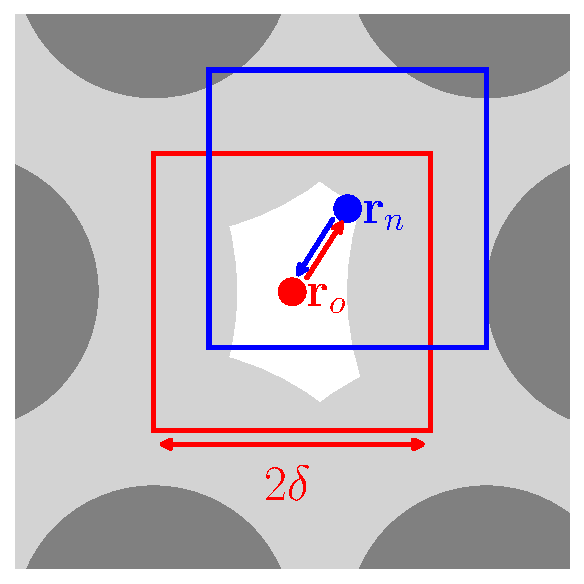
\includegraphics[width=4.5cm]{../figures/dccb_draw.pdf}
\caption{
An illustration of the old and new Rosenbluth terms for hard circles as described in Fig.~\ref{fig:lhs_nvt}.
The red box shows the positions available to $\pi_{cn}$ while the blue box shows the positions available to $\pi_{co}$.
Although the entire free volume is available to $\pi_{cn}$, it is not all available to $\pi_{co}$.
Thus, $\pi_{cn} \neq \pi_{co}$.
}
\label{fig:dccb_draw}
\end{centering}
\end{figure}

\begin{table}
\begin{center}
\begin{tabular}{|c|c|}
 \hline
 \thead{Forward} & \thead{$\alpha_{o\rightarrow n}$} \\ [0.5ex]
 \hline
 Choose from $N_m$ & $1/N_m$ \\
 \hline
 \makecell{Choose $c$ positions about $\mathbf{r}_o$.\\ Probability that $\mathbf{r}_n$ is in $c$.} & $c\diff\mathbf{r}/\delta^D$ \\
 \hline
 Choose $\mathbf{r}_n$ in $c$ positions & $\pi_{cn}$ \\
 \hline\hline
 \thead{Reverse} & \thead{$\alpha_{n\rightarrow o}$} \\ [0.5ex]
 \hline
 Choose from $N_m$ & $1/N_m$ \\
 \hline
 \makecell{Choose $c$ positions about $\mathbf{r}_n$.\\ Probability that $\mathbf{r}_o$ is in $c$.} & $c\diff\mathbf{r}/\delta^D$ \\
 \hline
 Choose $\mathbf{r}_o$ in $c$ positions & $\pi_{co}$ \\
 \hline
\end{tabular}
\caption{Translation with CB transition probabilities.}
\label{tab:lhs_disp_cb}
\end{center}
\end{table}

The transition probabilities are summarized in Table~\ref{tab:lhs_disp_cb}.
Using Table~\ref{tab:lhs_disp_cb} and substituting Eq.~\ref{eq:rhs_nvt} into Eq.~\ref{eq:detailed_balance}, the acceptance probability is
\begin{equation}
\chi = \frac{\pi_{co}}{\pi_{cn}}e^{-\beta \Delta U}.
\label{eq:cb}
\end{equation}

There is remarkable flexibility in the choice of $c$ positions, $\pi_{cn}$.
An often-used functional form is given by
\begin{equation}
\pi_{cn}=\frac{e^{-\beta U(\mathbf{r}_n)}}{W_{cn}},
\label{eq:pcn}
\end{equation}
where $W_{cn}=\sum_{in}^c e^{-\beta U(\mathbf{r}_{in})}$ and the subscript $in$ denotes that the positions, $\mathbf{r}_{in}$, were placed at random positions selected uniformly about $\mathbf{r}_o$ and contain $\mathbf{r}_n$.
Similarly, $\pi_{co}$ is given by
\begin{equation}
\pi_{co}=\frac{e^{-\beta U(\mathbf{r}_o)}}{W_{co}}
\label{eq:pco}
\end{equation}
where $W_{co}=\sum_{io}^c e^{-\beta U(\mathbf{r}_{io})}$ and the subscript $io$ denotes that the positions, $\mathbf{r}_{io}$, were placed at random positions selected uniformly about $\mathbf{r}_n$ and contain $\mathbf{r}_o$.

Substituting Eqs.~\ref{eq:pcn} and \ref{eq:pco} into Eq.~\ref{eq:cb} gives
\begin{equation}
\chi = \frac{W_{cn}}{W_{co}}e^{-\beta[\Delta U - U(\mathbf{r}_n) + U(\mathbf{r}_o)]}.
\end{equation}
This form of $\pi_{cn}$ is convenient because $\Delta U - U(\mathbf{r}_n) + U(\mathbf{r}_o)$ contains only interaction energies beyond the center of the first site (e.g., if there were multiple sites).

The efficiency of translation CB is debatable and depends upon the model system.
Standard translations for single-site isotropic particles described in Section~\ref{sec:lhs_translation} may be more optimal for the following reason.
Assuming that the calculation of the energy takes the majority of the CPU time, a standard translation requires computing the energy twice (or only once if the old contribution is stored).
In comparison, this choice of $\pi_{cn}$ and $\pi_{co}$ requires computing the energy $2c$ times (minus one if the old contribution is stored).
Thus, in the CPU time it takes to complete one of these CB trials, approximately $c$ standard trials could have been attempted, each with their own acceptance probability.
In this case, its possible more than one of the $c$ standard trials could have been accepted, in which case the standard approach would be more efficient.

On the other hand, other choices of $\pi_{cn}$ and $\pi_{co}$ could make CB translation efficient, even for single-site particles, as we will show in the next section.

%%%%%%%%%%%%%%%%%%%%%%%%%
\subsection{\label{sec:lhs_disp_dccb}Translation with dual-cut configurational bias (DCCB)}
%%%%%%%%%%%%%%%%%%%%%%%%%

A more efficient choice of $\pi_{cn}$ and $\pi_{co}$ is the DCCB approach if a suitable reference potential may be utilized \cite{vlugt_improving_1998}.
The namesake of DCCB is to apply a shorter cutoff to the energy calculation in $\pi_{cn}$ and $\pi_{co}$, but here we generalize dual-cut to include any reference potential, $U_r$, that takes less CPU time than the full potential, as discussed in Section~\ref{sec:lhs_insdel_cb}.
For DCCB,
\begin{equation}
\pi_{cn}=\frac{e^{-\beta U_r(\mathbf{r}_n)}}{W_{cnr}},
\label{eq:pcnr}
\end{equation}
where $W_{cnr}=\sum_{in}^c e^{-\beta U_r(\mathbf{r}_{in})}$ and the subscript $in$ denotes that the positions, $\mathbf{r}_{in}$, were placed at random positions selected uniformly about $\mathbf{r}_o$.
The acceptance criteria is then obtained by substituting Eq.~\ref{eq:pcnr} for both $\pi_{cn}$ and $\pi_{co}$ in Eq.~\ref{eq:cb},
\begin{equation}
\chi = \frac{W_{cnr}}{W_{cor}}e^{-\beta [\Delta U - U_r(\mathbf{r}_n) + U_r(\mathbf{r}_o)]}.
\end{equation}
Assuming that $U_r$ results in the choice of likely accepted configurations by approximating the highest-contributing parts of the full potential, the sampling efficiency may be increased.
On the other hand, a poor choice of $U_r$ could decrease the simulation efficiency.
In the worst case, ergodic sampling is broken by the rejection of valid configurations due to a poor reference potential, and the simulation results could be wrong.
Despite this, DCCB is an efficient method that may be tested and benchmarked against simulations without DCCB.

%%%%%%%%%%%%%%%%%%%%%%%%%
\subsection{\label{sec:lhs_cluster}Translation and rotation of rigid clusters}
%%%%%%%%%%%%%%%%%%%%%%%%%

The translation of rigid clusters is very similar to that of single particles described in Section~\ref{sec:lhs_translation}, except for the key differences that a cluster criteria must be specified, and that particles identified as part of a cluster must stay in that cluster after the trial.
If the clusters are allowed to change, then detailed balance is violated, as shown in Fig.~\ref{fig:cluster}.
Rigid cluster trial moves are biased because the transition probabilities depend on the configuration (i.e., the cluster criteria).

\begin{figure}
\begin{centering}
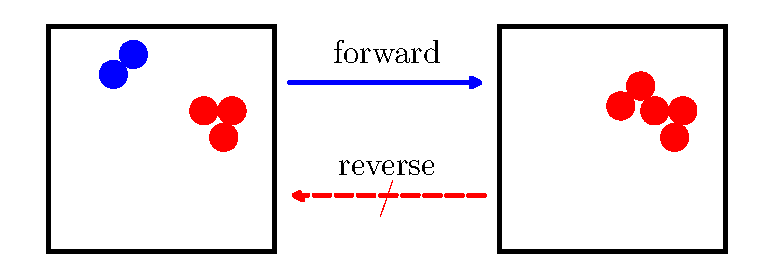
\includegraphics[width=6.5cm]{../figures/cluster.pdf}
\caption{
Detailed balance is violated if two separate clusters coalesce during a rigid cluster translation.
In the forward transition, the blue cluster is translated near a separate cluster shown in red.
If this move were allowed, the reverse cluster move would be impossible because clusters are moved rigidly and cannot be broken apart during the trial.
To obey detailed balance, reject rigid cluster moves that result in the coalescence of two originally separate clusters.
}
\label{fig:cluster}
\end{centering}
\end{figure}

A rigid cluster translation or rotation proceeds as follows.
First, an individual cluster is identified.
This identification could take many forms.
For example, one particle could be randomly chosen for a given type, and then a flood-fill algorithm could be used to find all particles within a distance cutoff from all particles in the cluster \cite{hatch_self-assembly_2016}.
Regardless of the metric used to identify clusters, the same metric must be applied again at the end of the trial.
In addition, if a cluster has picked up or lost any particles, then the trial must be immediately rejected.
Clusters may be rigidly translated or rotated with a parameter that is tunable during equilibration but must stay constant during production simulations, as described in Section~\ref{sec:lhs_translation}.
The acceptance criteria is then given by Eq.~\ref{eq:lhs_translate} or \ref{eq:lhs_rotate}.

%%%%%%%%%%%%%%%%%%%%%%%%%
\section{\label{sec:common_issues}Implementation issues in MC molecular simulations}
%%%%%%%%%%%%%%%%%%%%%%%%%

Although the derivation of the acceptance criteria for MC trials is the focus of this article, common errors encountered during the implementation of MC are included here.
For a more comprehensive discussion of the inner workings of MC see Ref.~\cite{dubbeldam_inner_2013}.
Thus, the scope of this section is for testing MC trial implementations.
In this section, we discuss energy tests and machine precision issues for helping to capture common errors, the calculation of standard deviations using the block method \cite{flyvbjerg_error_1989, grossfield_best_2018}, the generation of a random position on the surface of a unit sphere and spherical shell, and the generation of random rotation matrices.
This section then ends with a discussion of the general workflow for testing a new MC trial.

%%%%%%%%%%%%%%%%%%%%%%%%%
\subsection{\label{sec:energy_test}Energy tests and machine precision}
%%%%%%%%%%%%%%%%%%%%%%%%%

MC often involves the perturbation of a subset of the system instead of the entire system.
Only the energy of interaction of the perturbed particles needs to be computed to obtain the change in the energy of the system.
The energy of the system after a trial is accepted is the previous energy of the system plus the change.
This energy is referred to as the running total energy.
However, round off errors at the limit of numerical precision cause the running total energy to be different from the total energy calculated based on the interactions of all the particles.
This difference increases with the number of trials.
It is recommended to infrequently compute the energy of the entire system and compare the total energy with the running total energy from each energy change.
The total energy may also be compared and updated during trials which update all the particles, such as volume changes.
If the relative differences are not within an acceptable tolerance based on machine precision and the magnitude of the total energy, then this is a clear indication there is a problem with the way that the change in energy was computed, and an error or warning should be made visible.
If the relative difference is within an acceptable tolerance, the running total energy is then reset to the newly calculated value and the simulation continues.

Another recommended test is to not use any optimizations when infrequently computing the total energy of the entire system as part of the energy test described above.
Infrequent in this context essentially means much less often than once every $N$ trials, where $N$ is the total number of particles, assuming each trial moves individual particles, such that the computational cost of the trials is much greater than the computational cost of the infrequent and unoptimized total energy calculations.
If this unoptimized calculation of the entire system is done infrequently, it will not slow down the simulation significantly.
But it will serve as a test of the optimizations and may reveal issues with neighbor or cell lists, for example.

Machine precision round off errors may cause a number of other problems.
One that is frequently encountered in software implementations of MC is the acceptance probabilities.
Acceptance probabilities may involve several factors which are both big and small.
For this reason, it is best to compute and store acceptance probabilities as the natural logarithm, $\ln\chi$, and not $\chi$ \cite{shah_cassandra_2017}.
Machine precision issues may also appear when selecting among Rosenbluth weights.
In the FEASST \cite{hatch_monte_2024} implementation, overflow is avoided by shifting by a constant inside the exponential terms based on the maximum value, and later correcting for the shift.
Also, the total Rosenbluth factor may reveal if there is a very small chance for the trial to be accepted.
In that case, the trial may be outright rejected, because machine precision can make it difficult to select from among the poor choices.

%%%%%%%%%%%%%%%%%%%%%%%%%
\subsection{\label{sec:code}Additional code}
%%%%%%%%%%%%%%%%%%%%%%%%%

The following three sections contain Python code examples that were used in this article.
The first is for computing standard deviations of the mean using block averaging, which was utilized in the ideal gas tests to compare ensemble average properties with theoretical expectations.
The second is for randomly generating positions on a unit sphere, which is used for orienting molecules and anisotropic particles.
The third is for randomly generating positions in a spherical shell, which is used in AVB algorithms.

%%%%%%%%%%%%%%%%%%%%%%%%%
\subsubsection{\label{sec:block_av}Block averages}
%%%%%%%%%%%%%%%%%%%%%%%%%

In the example shown in Code Block~\ref{sim:statistics}, the standard deviation is computed using the blocking method \cite{flyvbjerg_error_1989}.
In this case, only blocks of $100$ samples are considered, but a careful analysis would show that the resulting standard deviation is independent of the block size (when large enough).
Thus, with this implementation, we are assuming that the sampled states are independent after $100$ MC trials, which may be reasonable for an ideal gas but most likely not for a dense liquid.
See the blocking tutorial in python interface of FEASST \cite{hatch_monte_2024} for an example with computing the block standard deviation from the average position of a particle randomly walking in one dimension with periodic boundary conditions.
If the maximum translation is smaller than the periodic boundary, correlations in the position may persist over many trials.

\begin{figure}
\lstinputlisting[
language=Python,
label={sim:statistics},
caption={The statistics module computes the mean and the standard deviation of the mean using blocks.}
]{../codes/statistics.py}
\end{figure}

%%%%%%%%%%%%%%%%%%%%%%%%%
\subsubsection{\label{sec:unit_sphere}Random position on a unit sphere surface and random orientation}
%%%%%%%%%%%%%%%%%%%%%%%%%

%In the example shown in Code Block~\ref{sim:unit_sphere}, positions are generated uniformly on the surface of a sphere.
%This is an important case to consider, because MC trials often assume that particles may be randomly oriented.
%However, one must be careful in how an orientation is generated.
%Uniformly selected values of Euler angles, for example, will result in a bias along the poles.
%Code Block~\ref{sim:quaternion} also shows how quaternions may be randomly generated to represent a uniformly random point on the surface of a sphere \cite{vesely_angular_1982}.
%Code Block~\ref{sim:rotationmatrix} uses these randomly generated quaternions to compute rotation matrices.
%A randomly generated perturbation of orientation is then demonstrated in Fig.~\ref{fig:random_orientation}.
Situations arise where one needs to generate a point at random uniformly on the surface of a sphere in 3D.  This is equivalent to defining an isotropically random direction or a randomly oriented unit vector. There are several ways to approach this: (1) sample the spherical coordinates $\theta$ and $\phi$, appropriately weighted; (2) use a rejection method to generate a point uniformly inside a sphere, i.e., repeatedly sample in a cube that circumscribes the sphere until the sample is also in the sphere, and then normalize the sampled point to a unit vector; (3) sample the $x$, $y$ and $z$ coordinates on independent Gaussian distributions, which yields a point sampled from a spherically symmetric 3D probability density, and normalize to a unit vector. The first method listed here is illustrated in Code Block~\ref{sim:unit_sphere}.

A similar problem is sampling a quaternion, which may be interpreted as a point on the surface of a unit 4D-hypersphere.
Accordingly, Code Block~\ref{sim:quaternion} shows how quaternions may be randomly generated by sampling uniformly on the surface of a 4D hypersphere using an efficient rejection method \cite{vesely_angular_1982}.
Code Block~\ref{sim:rotationmatrix} uses these randomly generated quaternions to compute rotation matrices, which could be used to generate a fully random orientation by rotating from an arbitrary reference orientation.
Finally, a randomly generated perturbation of orientation is shown using the axis-angle method in Code Block~\ref{sim:random_orientation} and Fig.~\ref{fig:random_orientation}.

\begin{figure}
\lstinputlisting[
language=Python,
label={sim:unit_sphere},
caption={The unit\_sphere module generates randomly uniform positions on the surface of a unit sphere in three dimensions.}
]{../codes/unit_sphere.py}
\end{figure}

\begin{figure}
\lstinputlisting[
language=Python,
label={sim:quaternion},
caption={The quaternion module generates a random quaternion by sampling on the surface of a 4-dimensional hypersphere.}
]{../codes/quaternion.py}
\end{figure}

\begin{figure}
\lstinputlisting[
language=Python,
label={sim:rotationmatrix},
caption={The rotation module generates a rotation matrix from an axis and angle or a quaternion. The first index is the row and the second index is the column, each starting with an index of zero.}
]{../codes/rotation.py}
\end{figure}

\begin{figure}
\lstinputlisting[
language=Python,
label={sim:random_orientation},
caption={Visualize randomly uniform perturbations in three dimensional particle orientations.}
]{../codes/random_orientation.py}
\end{figure}

\begin{figure}
\begin{centering}
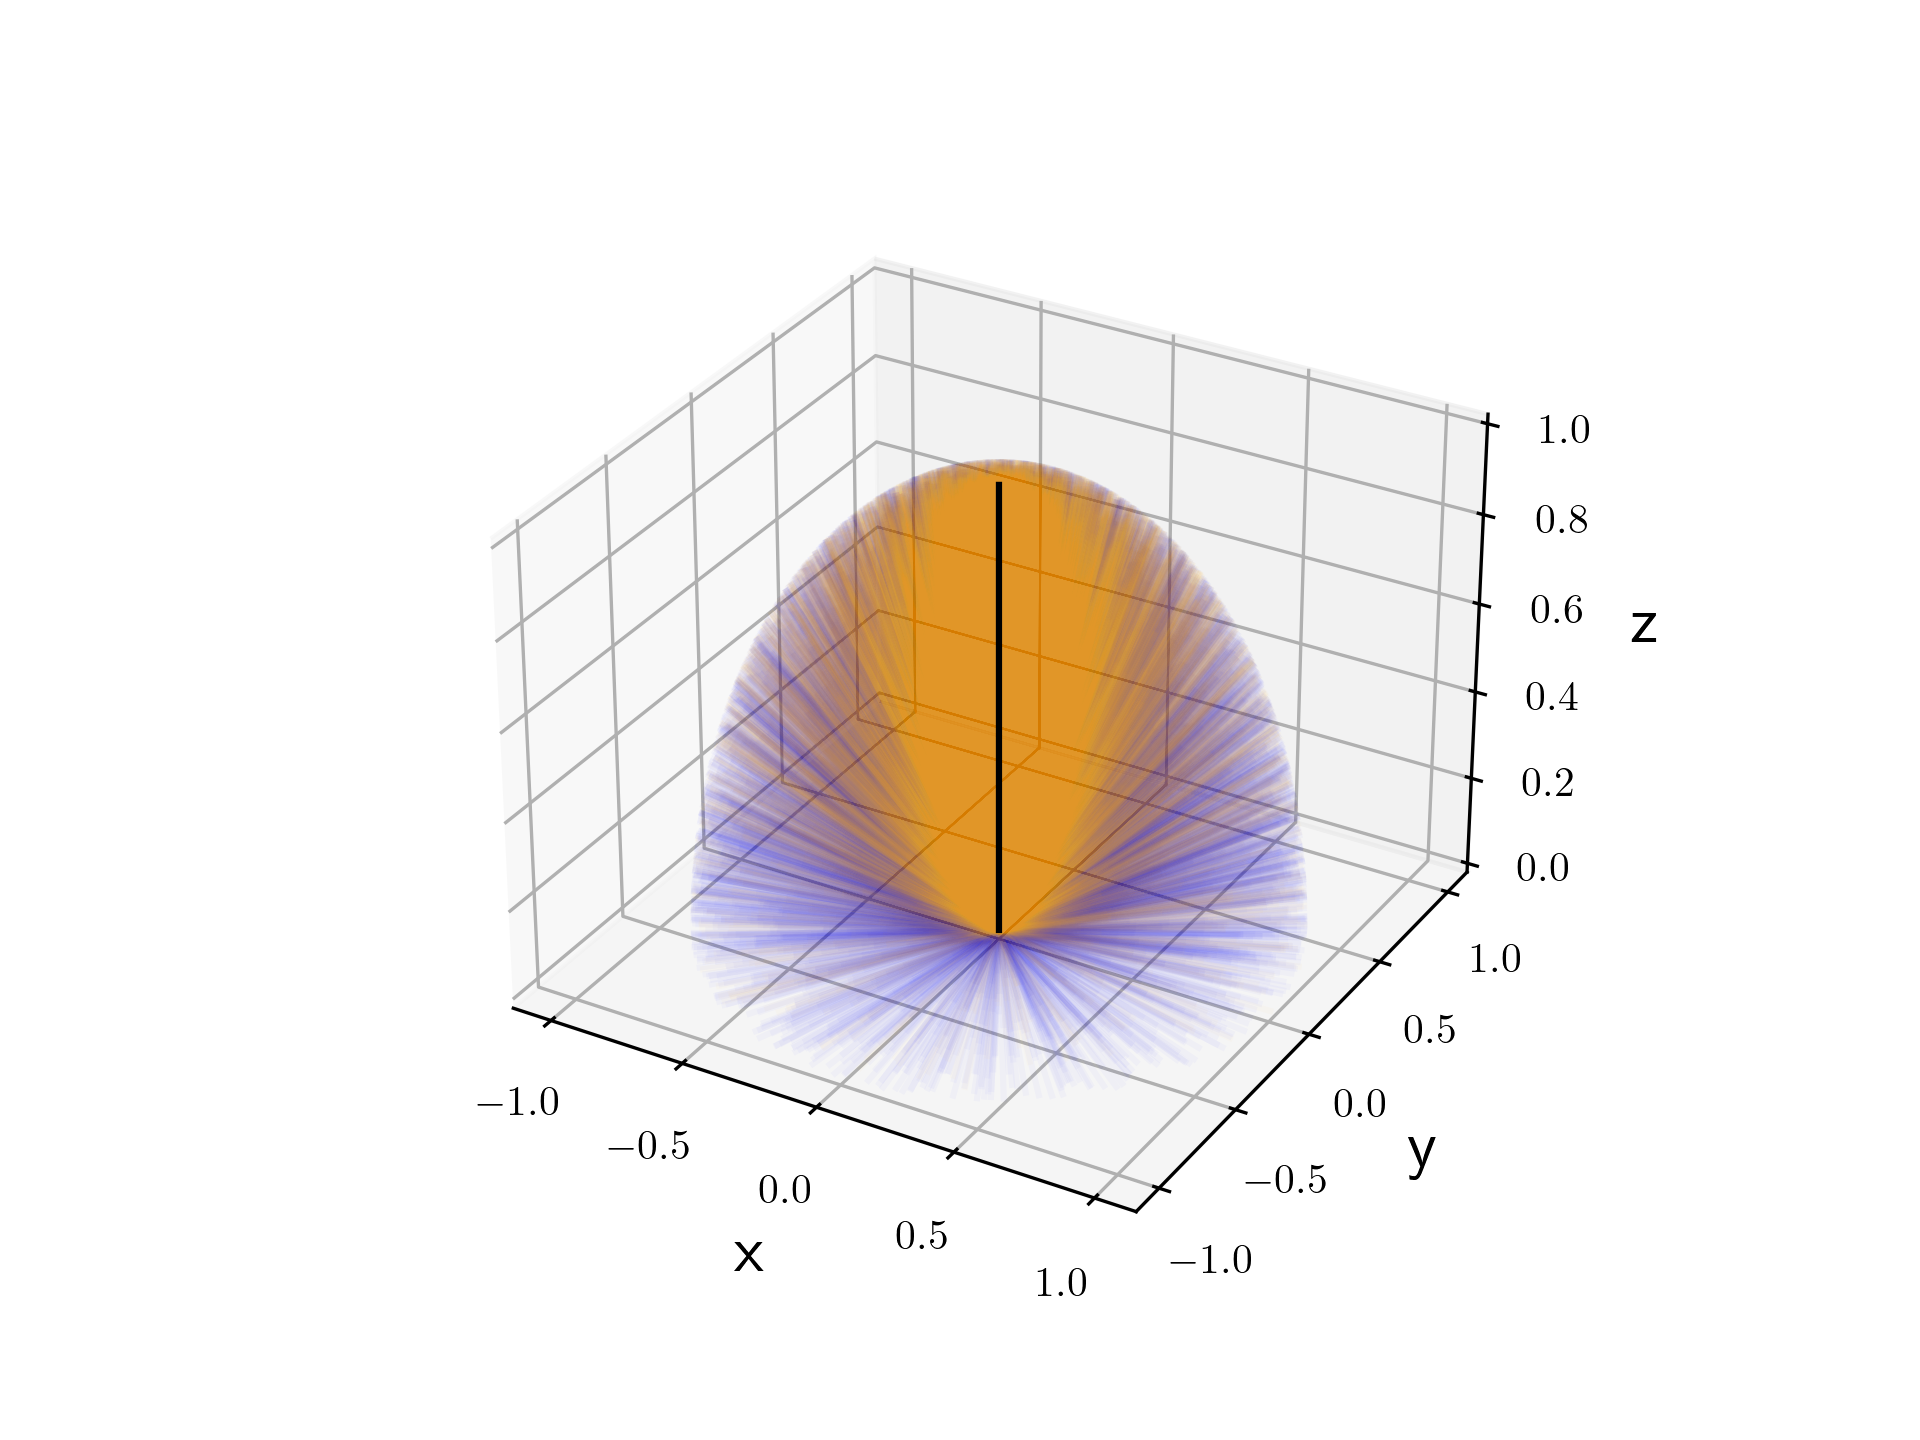
\includegraphics[width=8.5cm]{../figures/random_orientation.png}
\caption{
The output from Code Block~\ref{sim:random_orientation} shows $10^3$ uniformly random blue unit vectors emanating from the origin.
The other $10^3$ orange unit vectors are confined to the top hemisphere because they were randomly generated with the axis-angle method by perturbing the orientation of an upwards $z$-axis vector (shown in black) with a maximum angle parameter, $\delta \theta_{max}=\pi=180$ degrees.
\label{fig:random_orientation}
}
\end{centering}
\end{figure}

%%%%%%%%%%%%%%%%%%%%%%%%%
\subsubsection{\label{sec:spherical_shell}Uniform position in a spherical shell}
%%%%%%%%%%%%%%%%%%%%%%%%%

In the example shown in Code Block~\ref{sim:spherical_shell}, positions are generated uniformly within a spherical shell.
This is used to generate new trial positions with the AV of target isotropic sites, as shown in Fig.~\ref{fig:spherical_shell}.

\begin{figure}
\lstinputlisting[
language=Python,
label={sim:spherical_shell},
caption={Visualize randomly uniform positions in a spherical shell in three dimensions.}
]{../codes/spherical_shell.py}
\end{figure}

\begin{figure}
\begin{centering}

\includegraphics[width=8.5cm]{../figures/spherical_shell.png}
\caption{
Example output from Code Block~\ref{sim:spherical_shell} shows approximately $10^5$ small blue points randomly generated inside a spherical shell of outer radius $3$ and inner radius $2$.
To see the inside cavity, points above $z=0$ were removed.
\label{fig:spherical_shell}
}
\end{centering}
\end{figure}

%%%%%%%%%%%%%%%%%%%%%%%%%
\subsection{\label{sec:testingnewtrial}Workflow for testing a new MC trial}
%%%%%%%%%%%%%%%%%%%%%%%%%

Another recommendation during testing of new trials is to start with a result that was obtained using an established and well-tested set of trials and known to high confidence.
One source of such results is the National Institute of Standards and Technology (NIST) standard reference simulation website \cite{shen_nist_2017}.
Another choice is to generate results with one or more well-tested, open-source simulation codes.
Then, when computing the same result with the new trial, any differences may be further investigated.
Start with the simplest model and thermodynamic conditions that may reveal differences, such as an ideal gas simulation.
Also, if possible, completely remove as many other trials from the simulation with the new trial, thereby allowing one to better determine if the new trial is incorrect.
Otherwise, the difference in the results due to the new trial may be difficult to detect, or the impact of the new trial difficult to isolate, because the other trials are contributing greatly.
For example, AVB insertions and deletions can be tested without standard insertions and deletions, and without even $NVT$ translation and rotation trials.

%%%%%%%%%%%%%%%%%%%%%%%%%
\section{\label{sec:conc}Conclusions}
%%%%%%%%%%%%%%%%%%%%%%%%%

We provided a framework for deriving the Metropolis MC acceptance probabilities in the $NVT$, $NPT$, (semi)-$\mu VT$ and Gibbs ensembles with a detailed checklist for generating unbiased trials in each of these ensembles.
Discussions of how detailed balance may be violated, as well as code examples to compare ideal gas MC results with theoretical predictions, were provided.
The checklist was applied with a table format for generating the transition probabilities to help reduce errors.
We considered complex trials with bias, which include the illustrations and tables but not code examples.
Finally, a discussion of common implementation issues in MC were included, along with code examples.
It is our hope that this article will make MC molecular simulation methodology development more accessible in general to researchers.
When implementing complex MC trials, we recommend first testing with a number of models and thermodynamic conditions, starting with the simplest and fastest ideal gas simulation.

We encourage readers to comment upon this guide using the issue tracker of the GitHub repository [\url{https://github.com/usnistgov/best-practices-mc}].
There are many more methods we would like to add to this guide.
Future versions may include the following MC methods: orientation bias, Mayer sampling, expanded ensembles, geometric cluster algorithm, shell particles, bond, angle and branch algorithms and tests.
%k=0 for sin(theta) distributions according to random point picking.

%%%%%%%%%%%%%%%%%%%%%%%%%
\section{\label{sec:ack}Acknowledgements and Disclaimer}
%%%%%%%%%%%%%%%%%%%%%%%%%

This article was funded by NIST and is not subject to U.S. Copyright.
Certain commercial firms and trade names are identified in order to specify the usage procedures adequately for reproducibility.
Such identification is not intended to imply recommendation or endorsement by the National Institute of Standards and Technology, nor is it intended to imply that related products are necessarily the best available for the purpose.

\section*{Author Information}
\makeorcid

\nocite{*}
\bibliography{paper}
\end{document}
